% Article of the repository (milestone M17, docs/tasks/M17-article.md).
% Narrative only: every number, table, figure and the milestone status come from the
% macros of generated.tex (\chiffre, \articletable, \articlefig, \articleetat…), rewritten
% by `make article`. Never type a result by hand: `python -m tools.article --check`
% (make ci) rejects a decimal number written in the abstract or in sections 4 to 10.
% PDF: `make article-pdf` (xelatex + bibtex) → docs/article/article.pdf.
\documentclass[11pt,a4paper]{article}

\usepackage{fontspec}
\usepackage[margin=2.2cm]{geometry}
\usepackage{amsmath,amssymb}
\usepackage{graphicx}
\usepackage{booktabs,tabularx,array}
\usepackage[font=small,labelfont=bf]{caption}
\usepackage{xcolor}
\usepackage[numbers,square,sort]{natbib}
\usepackage[colorlinks=true,linkcolor=blue!50!black,citecolor=green!35!black,
            urlcolor=blue!50!black]{hyperref}
\usepackage{enumitem}
\setlist{nosep,leftmargin=*}
\setlength{\parskip}{0.35em}
\renewcommand{\arraystretch}{1.12}

% Generated by `python -m tools.article render` (make article): do not edit by hand.
% Numbers: docs/article/chiffres.json; figures: tools/figures; status: docs/tasks/README.md.
\newcommand\artget[2]{\ifcsname art#1:#2\endcsname\csname art#1:#2\endcsname
  \else\PackageError{article}{unknown #1 key '#2' (make article)}{}\fi}
\newcommand\chiffre[1]{\artget{n}{#1}}
\newcommand\articletable[1]{\artget{table}{#1}}
\newcommand\articlefig[1]{\artget{fig}{#1}}

% ---- numbers
\expandafter\def\csname artn:balayage.crowdhuman.meilleur.map\endcsname{%
35.87\textsuperscript{tier R}}  % tier-R, docs/tasks/resultats-balayages.md
\expandafter\def\csname artn:balayage.exdark.meilleur.map\endcsname{%
13.29\textsuperscript{tier R}}  % tier-R, docs/tasks/resultats-balayages.md
\expandafter\def\csname artn:balayage.flir.meilleur.map\endcsname{%
0.70\textsuperscript{tier R}}  % tier-R, docs/tasks/resultats-balayages.md
\expandafter\def\csname artn:balayage.kitti.meilleur.map\endcsname{%
2.38\textsuperscript{tier R}}  % tier-R, docs/tasks/resultats-balayages.md
\expandafter\def\csname artn:balayage.visdrone.meilleur.map\endcsname{%
2.24\textsuperscript{tier R}}  % tier-R, docs/tasks/resultats-balayages.md
\expandafter\def\csname artn:balayage.voc.meilleur.map\endcsname{%
36.27\textsuperscript{tier R}}  % tier-R, docs/tasks/resultats-balayages.md
\expandafter\def\csname artn:map.formats.admm\endcsname{%
43.07}  % measured, results/req_yolo.md
\expandafter\def\csname artn:map.formats.hwpp\endcsname{%
55.56}  % measured, results/postproc_hw.md
\expandafter\def\csname artn:map.formats.mixed6\endcsname{%
52.46}  % measured, results/req_yolo.md
\expandafter\def\csname artn:map.formats.uniform6\endcsname{%
54.35}  % measured, results/req_yolo.md
\expandafter\def\csname artn:map.formats.w4a4.ptq\endcsname{%
17.06}  % measured, results/quant_4bits.md
\expandafter\def\csname artn:map.formats.w4a4.qat\endcsname{%
36.38}  % measured, results/quant_4bits.md
\expandafter\def\csname artn:map.voc.csim\endcsname{%
55.66\textsuperscript{C-sim}}  % csim, results/map_stades.md
\expandafter\def\csname artn:map.voc.darknet\endcsname{%
57.1\textsuperscript{pub.}}  % published, results/map_float.md
\expandafter\def\csname artn:map.voc.drop\endcsname{%
−0.64}  % measured, results/map_stades.md
\expandafter\def\csname artn:map.voc.float\endcsname{%
56.30}  % measured, results/map_stades.md
\expandafter\def\csname artn:map.voc.identical\endcsname{%
4,952\textsuperscript{C-sim}}  % csim, results/map_stades.md
\expandafter\def\csname artn:map.voc.images\endcsname{%
4,952}  % measured, results/map_stades.md
\expandafter\def\csname artn:map.voc.int8\endcsname{%
55.66}  % measured, results/map_stades.md
\expandafter\def\csname artn:model.v2.gmacs\endcsname{%
3.49}  % measured, python/yolo/models/specs.py
\expandafter\def\csname artn:model.v2.mparams\endcsname{%
15.86}  % measured, python/yolo/models/specs.py
\expandafter\def\csname artn:model.v3.gmacs\endcsname{%
2.74}  % measured, python/yolo/models/specs.py
\expandafter\def\csname artn:model.v3.mparams\endcsname{%
8.71}  % measured, python/yolo/models/specs.py
\expandafter\def\csname artn:perf.kv260.bound.ms\endcsname{%
31.6\textsuperscript{proj.}}  % projection, results/rapport.md
\expandafter\def\csname artn:perf.kv260.m6.ms\endcsname{%
206.5\textsuperscript{proj.}}  % projection, results/rapport.md
\expandafter\def\csname artn:perf.kv260.roofline.ms\endcsname{%
31.9\textsuperscript{proj.}}  % projection, results/rapport.md
\expandafter\def\csname artn:perf.kv260.v2.eff\endcsname{%
61.0\textsuperscript{proj.}}  % projection, results/mesures.md
\expandafter\def\csname artn:perf.kv260.v2.fps\endcsname{%
26.9\textsuperscript{proj.}}  % projection, results/mesures.md
\expandafter\def\csname artn:perf.kv260.v2.gops\endcsname{%
187.3\textsuperscript{proj.}}  % projection, results/mesures.md
\expandafter\def\csname artn:perf.kv260.v2.ms\endcsname{%
37.2\textsuperscript{proj.}}  % projection, results/mesures.md
\expandafter\def\csname artn:perf.kv260.v3.ms\endcsname{%
36.1\textsuperscript{proj.}}  % projection, results/mesures.md
\expandafter\def\csname artn:quant.sensitive.gap\endcsname{%
−0.61\textsuperscript{tier R}}  % tier-R, results/map_int8.md
\expandafter\def\csname artn:quant.sensitive.layer\endcsname{%
L10\textsuperscript{tier R}}  % tier-R, results/map_int8.md
\expandafter\def\csname artn:stream.w4.fps\endcsname{%
64.2\textsuperscript{est.}}  % estimate, results/streaming.md
\expandafter\def\csname artn:stream.w8.dsp\endcsname{%
968\textsuperscript{est.}}  % estimate, results/streaming.md
\expandafter\def\csname artn:stream.w8.fps\endcsname{%
32.1\textsuperscript{est.}}  % estimate, results/streaming.md
\expandafter\def\csname artn:stream.w8.latency\endcsname{%
85.2\textsuperscript{est.}}  % estimate, results/streaming.md
\expandafter\def\csname artn:verif.dumps\endcsname{%
6}  % measured, Makefile (DUMP_IMAGES × QNETS)
\expandafter\def\csname artn:verif.hwpp.cases\endcsname{%
1,014\textsuperscript{C-sim}}  % csim, results/postproc_hw.md
% ---- tables
\expandafter\def\csname arttable:balayages.meilleurs\endcsname{%
\setlength{\tabcolsep}{4pt}
\begin{tabularx}{\linewidth}{@{}>{\raggedright\arraybackslash}Xr>{\raggedright\arraybackslash}Xr>{\raggedright\arraybackslash}X>{\raggedright\arraybackslash}Xr>{\raggedright\arraybackslash}X@{}}
\toprule
\textbf{Dataset} & \textbf{\begin{tabular}[b]{@{}r@{}}Training\\images\end{tabular}} & \textbf{Best run} & \textbf{Batch} & \textbf{Training subset} & \textbf{Metric} & \textbf{\begin{tabular}[b]{@{}r@{}}Score (50\\images)\end{tabular}} & \textbf{Status} \\
\midrule
VOC & 16,551 & \texttt{b32-sall} & 32 & all & mAP, 11 points & 36.27 & tier-R \\
VisDrone & 6,471 & \texttt{b32-sall} & 32 & all & mAP, 11 points & 2.24 & tier-R \\
KITTI & 5,985 & \texttt{b32-sall} & 32 & all & mAP, 11 points & 2.38 & tier-R \\
FLIR & 10,742 & \texttt{b8-sall} & 8 & all & AP@[.5:.95] (COCO) & 0.70 & tier-R \\
ExDark & 3,000 & \texttt{b32-sall} & 32 & all & mAP, 11 points & 13.29 & tier-R \\
CrowdHuman & 15,000 & \texttt{b16-sall} & 16 & all & mAP, 11 points & 35.87 & tier-R \\
\bottomrule
\end{tabularx}}
\expandafter\def\csname arttable:benchmarks\endcsname{%
\setlength{\tabcolsep}{4pt}
\begin{tabularx}{\linewidth}{@{}>{\raggedright\arraybackslash}X>{\raggedright\arraybackslash}X>{\raggedright\arraybackslash}X>{\raggedright\arraybackslash}X>{\raggedright\arraybackslash}X>{\raggedright\arraybackslash}X>{\raggedright\arraybackslash}X>{\raggedright\arraybackslash}X>{\raggedright\arraybackslash}X@{}}
\toprule
\textbf{Work} & \textbf{Model} & \textbf{FPGA} & \textbf{Format} & \textbf{img/s} & \textbf{ms} & \textbf{GOPS} & \textbf{W} & \textbf{Status} \\
\midrule
2023-zhai & YOLOv3-tiny pruned, 1 module & Zynq XC7Z035 & INT16 & 91.65 & — & 67.91 & 12.51 & published \\
2023-zhai & YOLOv3-tiny pruned, 2 modules & Zynq XC7Z035 & INT16 & 168.72 & — & 124.01 & 15.18 & published \\
2024-zhang & YOLOv2-Tiny 416, batch 1 & Kintex-7 325T & INT8 & — & 14.49 & 406 & 12.3 & published \\
2024-zhang & YOLOv3-Tiny 416, batch 1 & Kintex-7 325T & INT8 & — & 15.2 & 401 & 12.3 & published \\
2023-montgomerie-corcoran & YOLOv3-Tiny 416 & VCU110 & W8A16 & — & — & 418.9 & 15.4 & published \\
2019-ding & Tiny-YOLOv2, ADMM heterogeneous & Virtex-7 690T & FFT + powers of 2 & 314.2 & — & — & 21 & published \\
2026-fata & YOLOv3-tiny pruned at 70 \% (DPU Vitis AI) & Kria KV260 (DPU) & INT8 QAT & 24.3 & — & 60.18 & 2.13 & published \\
2025-kim & YOLOv2 full (prototype) & Zybo Z7-20 & INT16 & 0.083 & 12,000 & — & — & published \\
this work (C-sim projection) & Tiny-YOLOv2 VOC 416 & Kria KV260 (XCK26) & INT8 (W8A8, per channel) & 26.87 & 37.2 & 187.3 & — & projection \\
this work (C-sim projection) & Tiny-YOLOv3 COCO 416 & Kria KV260 (XCK26) & INT8 (W8A8, per channel) & 27.72 & 36.1 & 154.3 & — & projection \\
\bottomrule
\end{tabularx}}
\expandafter\def\csname arttable:map.formats\endcsname{%
\setlength{\tabcolsep}{4pt}
\begin{tabularx}{\linewidth}{@{}>{\raggedright\arraybackslash}X>{\raggedright\arraybackslash}Xrr@{}}
\toprule
\textbf{Weights / activations} & \textbf{Method} & \textbf{mAP} & \textbf{\begin{tabular}[b]{@{}r@{}}Gap to\\INT8\end{tabular}} \\
\midrule
INT8 per channel (reference) & PTQ & 55.66 & — \\
uniform6 (±31) & PTQ & 54.35 & −1.31 \\
mixed6 (powers of 2) & PTQ, direct projection & 52.46 & −3.20 \\
mixed6 & ADMM, 600 iterations, then projection & 43.07 & −12.59 \\
w4a4 & PTQ (power-of-2 steps) & 17.06 & −38.60 \\
w4a4 & QAT, 600 iterations & 36.38 & −19.28 \\
INT8 + hardware post-processing & unsorted NMS, Q4 boxes & 55.56 & −0.10 \\
\bottomrule
\end{tabularx}}
\expandafter\def\csname arttable:map.stades\endcsname{%
\setlength{\tabcolsep}{4pt}
\begin{tabularx}{\linewidth}{@{}>{\raggedright\arraybackslash}Xr>{\raggedright\arraybackslash}X>{\raggedright\arraybackslash}X@{}}
\toprule
\textbf{Stage} & \textbf{mAP} & \textbf{Equality with the integer model} & \textbf{Status} \\
\midrule
Float (fused BN, NumPy float32) & 56.30 & — & measured \\
Integer, Python (\texttt{IntNetwork}, bit-exact) & 55.66 & reference & measured \\
FPGA, C-sim (ARM driver, sim backend, PC) & 55.66 & 4,952 / 4,952 identical images & csim \\
FPGA, KV260 (uio backend) & — & to be measured & — \\
\bottomrule
\end{tabularx}}
\expandafter\def\csname arttable:map.voc.float.table\endcsname{%
\setlength{\tabcolsep}{4pt}
\begin{tabularx}{\linewidth}{@{}>{\raggedright\arraybackslash}X>{\raggedright\arraybackslash}Xr@{}}
\toprule
\textbf{Preprocessing} & \textbf{Interpolation} & \textbf{mAP} \\
\midrule
direct resize (\texttt{stretch}) & Pillow bilinear & 56.30 \\
direct resize (\texttt{stretch}) & Darknet (\texttt{resize\_image}) & 56.32 \\
letterbox & Pillow bilinear & 54.18 \\
letterbox & Darknet (\texttt{resize\_image}) & 53.98 \\
\bottomrule
\end{tabularx}}
\expandafter\def\csname arttable:map.voc.int8.table\endcsname{%
\setlength{\tabcolsep}{4pt}
\begin{tabularx}{\linewidth}{@{}>{\raggedright\arraybackslash}Xrrr@{}}
\toprule
\textbf{Preprocessing} & \textbf{\begin{tabular}[b]{@{}r@{}}Float\\(fused BN)\end{tabular}} & \textbf{\begin{tabular}[b]{@{}r@{}}Integer\\INT8\end{tabular}} & \textbf{Gap} \\
\midrule
stretch (\texttt{make eval-float}) & 56.30 & 55.66 & −0.64 \\
letterbox (the training one) & 54.18 & 53.68 & −0.50 \\
\bottomrule
\end{tabularx}}
\expandafter\def\csname arttable:perf.cascade\endcsname{%
\setlength{\tabcolsep}{4pt}
\begin{tabularx}{\linewidth}{@{}>{\raggedright\arraybackslash}Xrrrrr@{}}
\toprule
\textbf{Kernel configuration (Tiny-YOLOv2)} & \textbf{Mcycles} & \textbf{ms} & \textbf{img/s} & \textbf{GOPS} & \textbf{\begin{tabular}[b]{@{}r@{}}MAC efficiency\\(\%)\end{tabular}} \\
\midrule
M6: ports 8 bits & 41.30 & 206.5 & 4.8 & 33.8 & 11.0 \\
valid channels only (trim) & 32.67 & 163.3 & 6.1 & 42.7 & 13.9 \\
ports 64 bits & 12.27 & 61.3 & 16.3 & 113.6 & 37.0 \\
ports 128 bits + trim & 12.13 & 60.6 & 16.5 & 115.0 & 37.4 \\
ports 64 bits + trim + requantization ×8 (+28 DSP) & 9.29 & 46.4 & 21.5 & 150.1 & 48.9 \\
... + L00 folding & 8.38 & 41.9 & 23.9 & 166.4 & 54.2 \\
... + 14×14 tiles for pooled convs (M10 kernel) & 7.44 & 37.2 & 26.9 & 187.3 & 61.0 \\
compute bound of M6 (free loads) & 8.23 & 41.1 & 24.3 & 169.5 & 55.2 \\
compute bound of the M10 kernel & 6.32 & 31.6 & 31.7 & 220.7 & 71.8 \\
KV260 roofline point (roofline.md) & — & 31.9 & 31.3 & 218.5 & — \\
ideal (MACs / 768, efficiency 100 \%) & 4.54 & 22.7 & 44.1 & 307.2 & 100.0 \\
\bottomrule
\end{tabularx}
\par\smallskip{\footnotesize\emph{Status of every number of this table: projection.}}}
\expandafter\def\csname arttable:perf.kv260\endcsname{%
\setlength{\tabcolsep}{4pt}
\begin{tabularx}{\linewidth}{@{}>{\raggedright\arraybackslash}Xrrrrrr>{\raggedright\arraybackslash}X@{}}
\toprule
\textbf{Network} & \textbf{GMAC} & \textbf{Mcycles} & \textbf{ms} & \textbf{img/s} & \textbf{GOPS} & \textbf{\begin{tabular}[b]{@{}r@{}}MAC efficiency\\(\%)\end{tabular}} & \textbf{Status} \\
\midrule
\texttt{tiny-yolov2-voc} & 3.486 & 7.44 & 37.2 & 26.9 & 187.3 & 61.0 & projection \\
\texttt{tiny-yolov3-coco} & 2.782 & 7.21 & 36.1 & 27.7 & 154.3 & 50.2 & projection \\
\bottomrule
\end{tabularx}}
% ---- figures cited by article.tex
\expandafter\def\csname artfig:etat_art\endcsname{%
\begin{figure}[htbp]
\centering
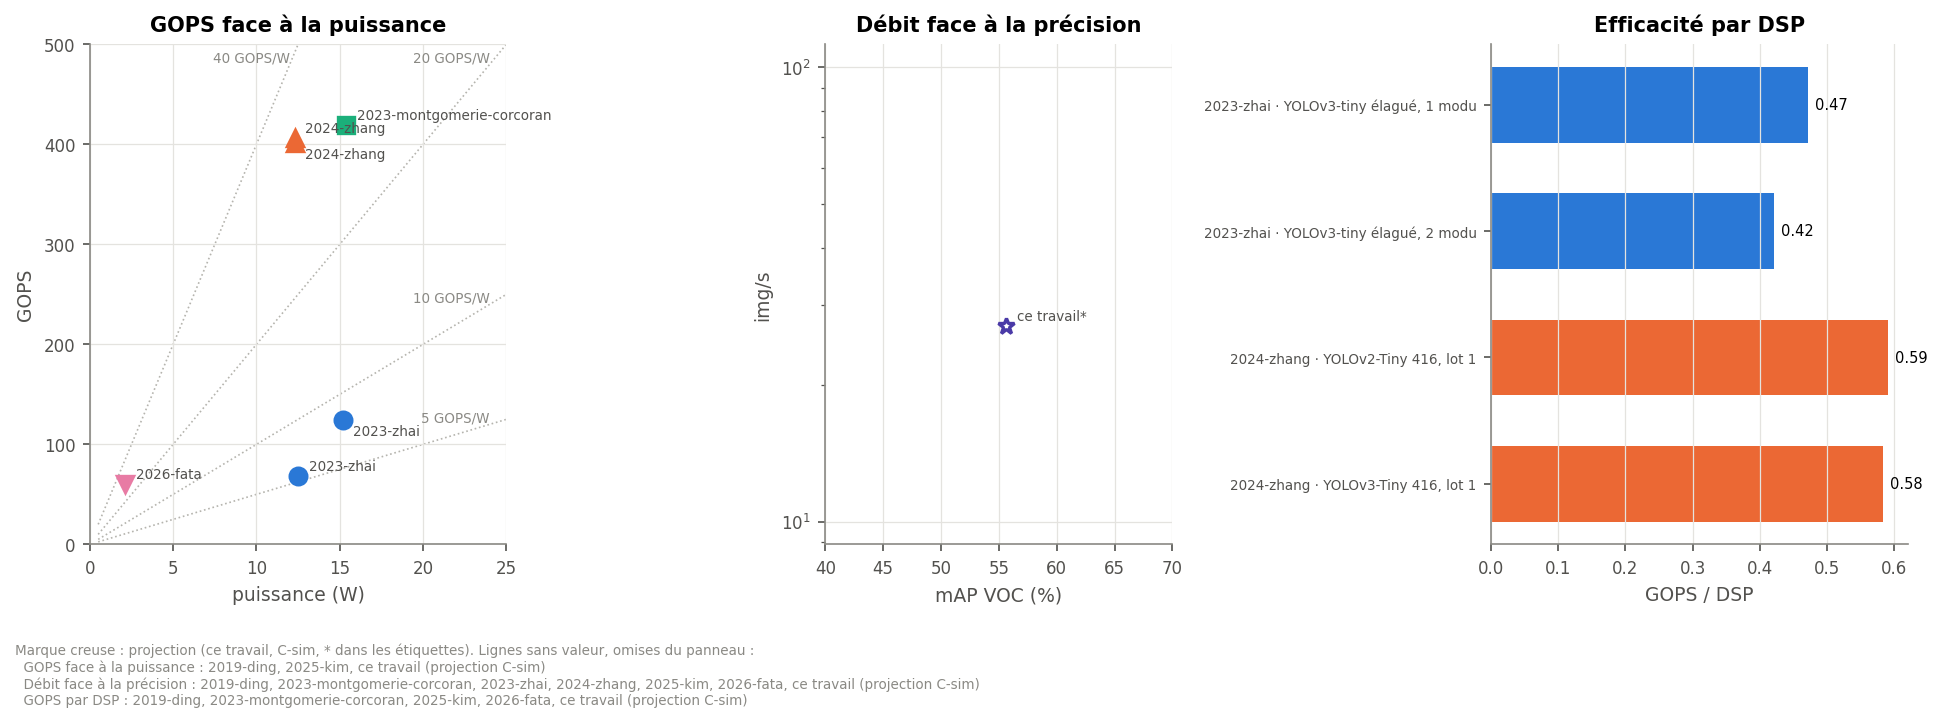
\includegraphics[width=\linewidth,height=0.42\textheight,keepaspectratio]{../../results/figures/resultats/etat_art.png}
\caption{Comparaison aux accélérateurs publiés : GOPS et puissance, débit et mAP, GOPS par DSP (marque creuse : projection de ce travail). (\texttt{etat\_art})}
\label{fig:etat_art}
% python -m tools.figures etat_art
\end{figure}}
\expandafter\def\csname artfig:graphe/graphe_tiny-yolov2-voc\endcsname{%
\begin{figure}[htbp]
\centering
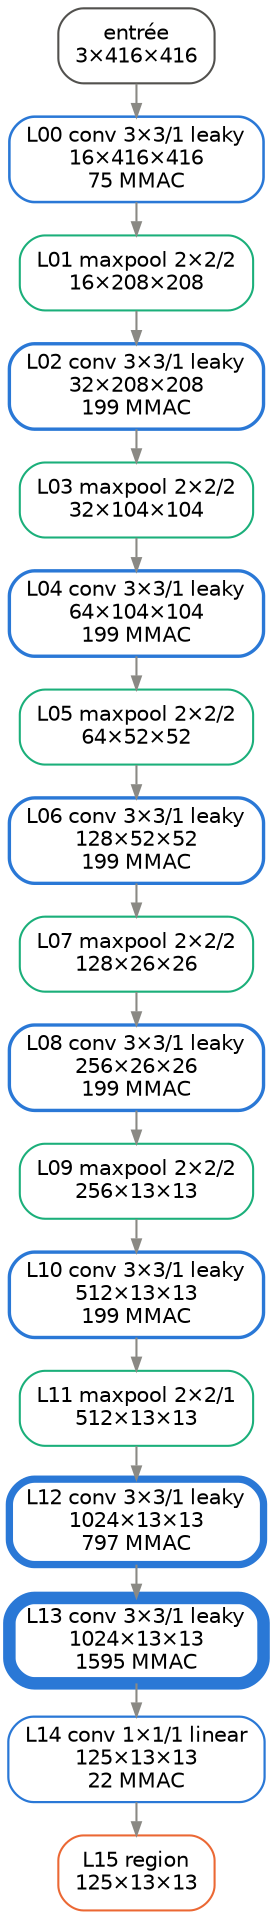
\includegraphics[width=\linewidth,height=0.42\textheight,keepaspectratio]{../../results/figures/modeles/graphe_tiny-yolov2-voc.png}
\caption{Graphe couche par couche (type, noyau et stride, forme de sortie C×H×W ; bord épais = beaucoup de MACs). (\texttt{graphe})}
\label{fig:graphe/graphe_tiny-yolov2-voc}
% python -m tools.figures graphe
\end{figure}}
\expandafter\def\csname artfig:fiche/fiche_tiny-yolov2-voc\endcsname{%
\begin{figure}[htbp]
\centering
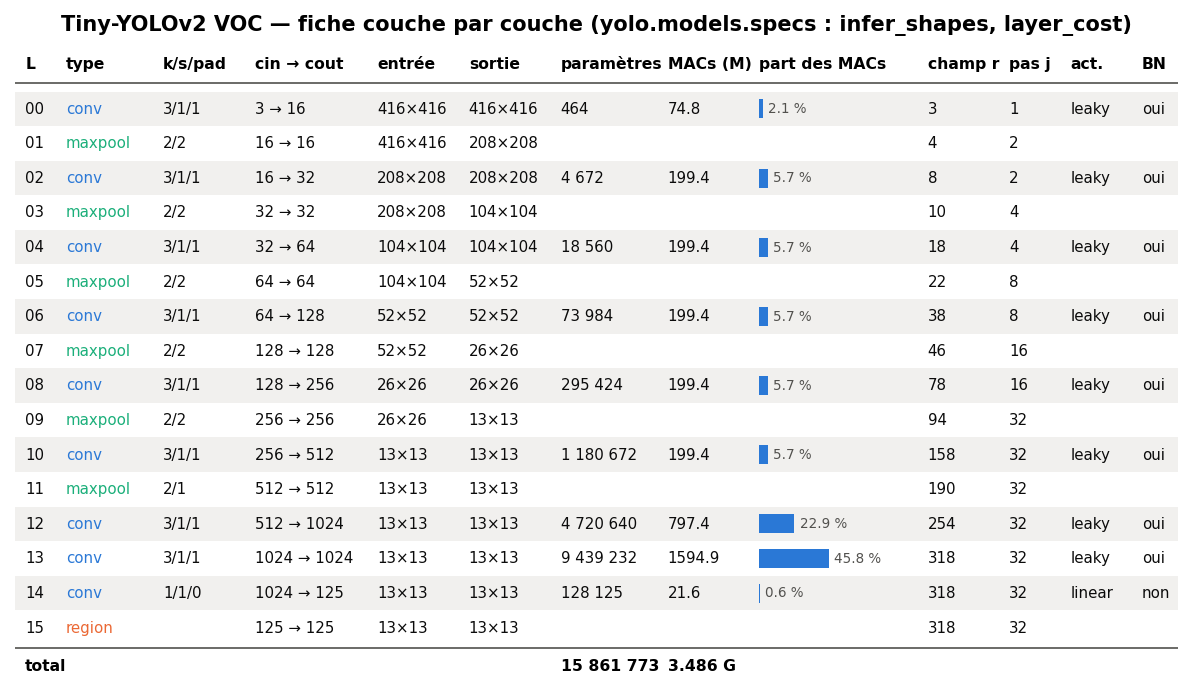
\includegraphics[width=\linewidth,height=0.42\textheight,keepaspectratio]{../../results/figures/reseaux/fiche_tiny-yolov2-voc.png}
\caption{Fiche couche par couche : type, noyau, formes, paramètres, MACs et leur part, champ réceptif et pas cumulé (CSV à côté de l'image). (\texttt{fiche})}
\label{fig:fiche/fiche_tiny-yolov2-voc}
% python -m tools.figures fiche
\end{figure}}
\expandafter\def\csname artfig:convolution\endcsname{%
\begin{figure}[htbp]
\centering
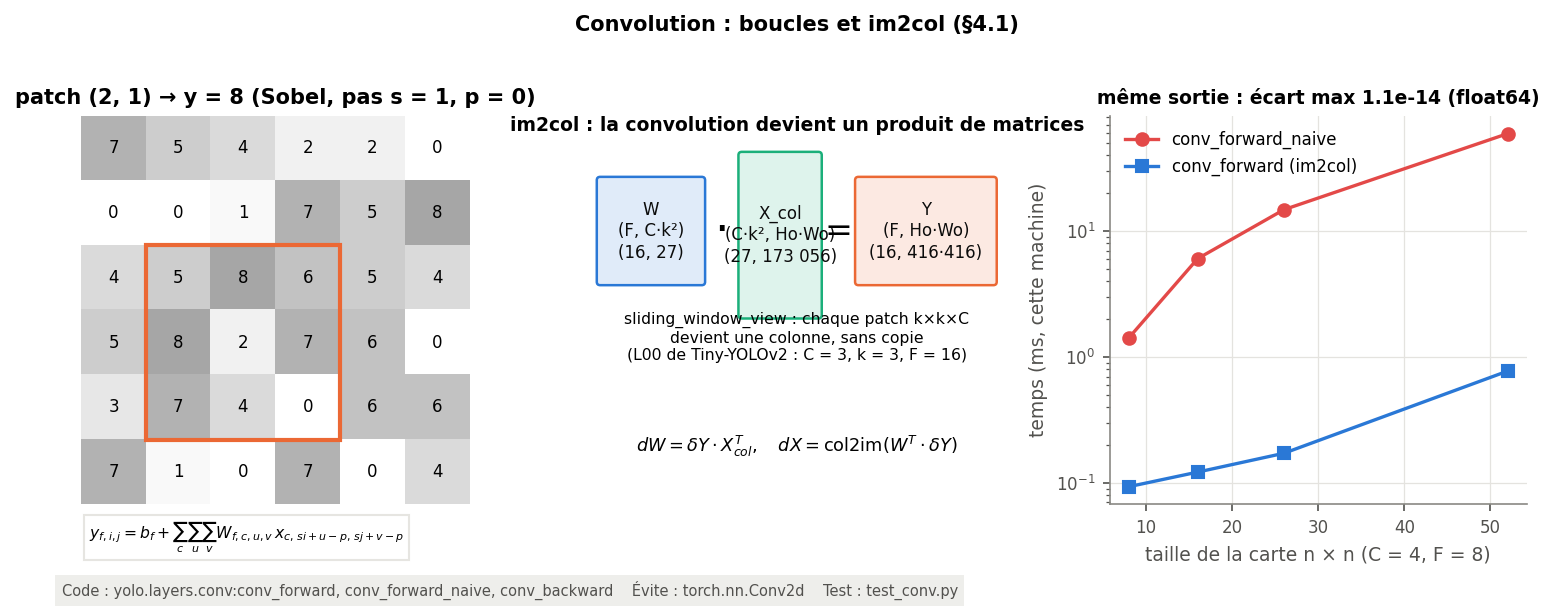
\includegraphics[width=\linewidth,height=0.42\textheight,keepaspectratio]{../../results/figures/maths/convolution.png}
\caption{Convolution : la formule sur un patch, le dépliage im2col en produit de matrices, et le temps des boucles face à im2col. (\texttt{convolution})}
\label{fig:convolution}
% python -m tools.figures convolution
\end{figure}}
\expandafter\def\csname artfig:retropropagation\endcsname{%
\begin{figure}[htbp]
\centering
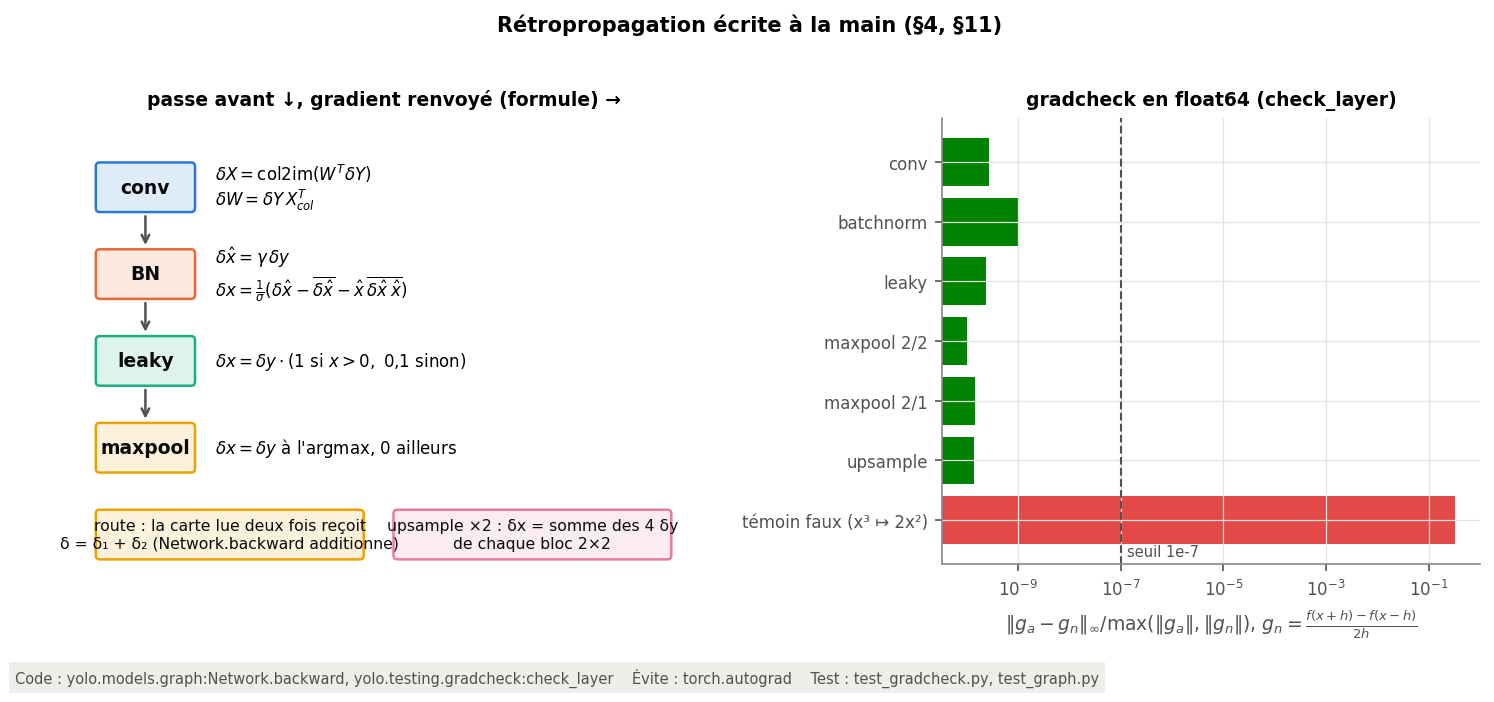
\includegraphics[width=\linewidth,height=0.42\textheight,keepaspectratio]{../../results/figures/maths/retropropagation.png}
\caption{Rétropropagation écrite à la main : formule du gradient renvoyé par chaque couche, puis l'erreur du gradcheck par couche face au seuil 1e-7. (\texttt{retropropagation})}
\label{fig:retropropagation}
% python -m tools.figures retropropagation
\end{figure}}
\expandafter\def\csname artfig:perte\endcsname{%
\begin{figure}[htbp]
\centering
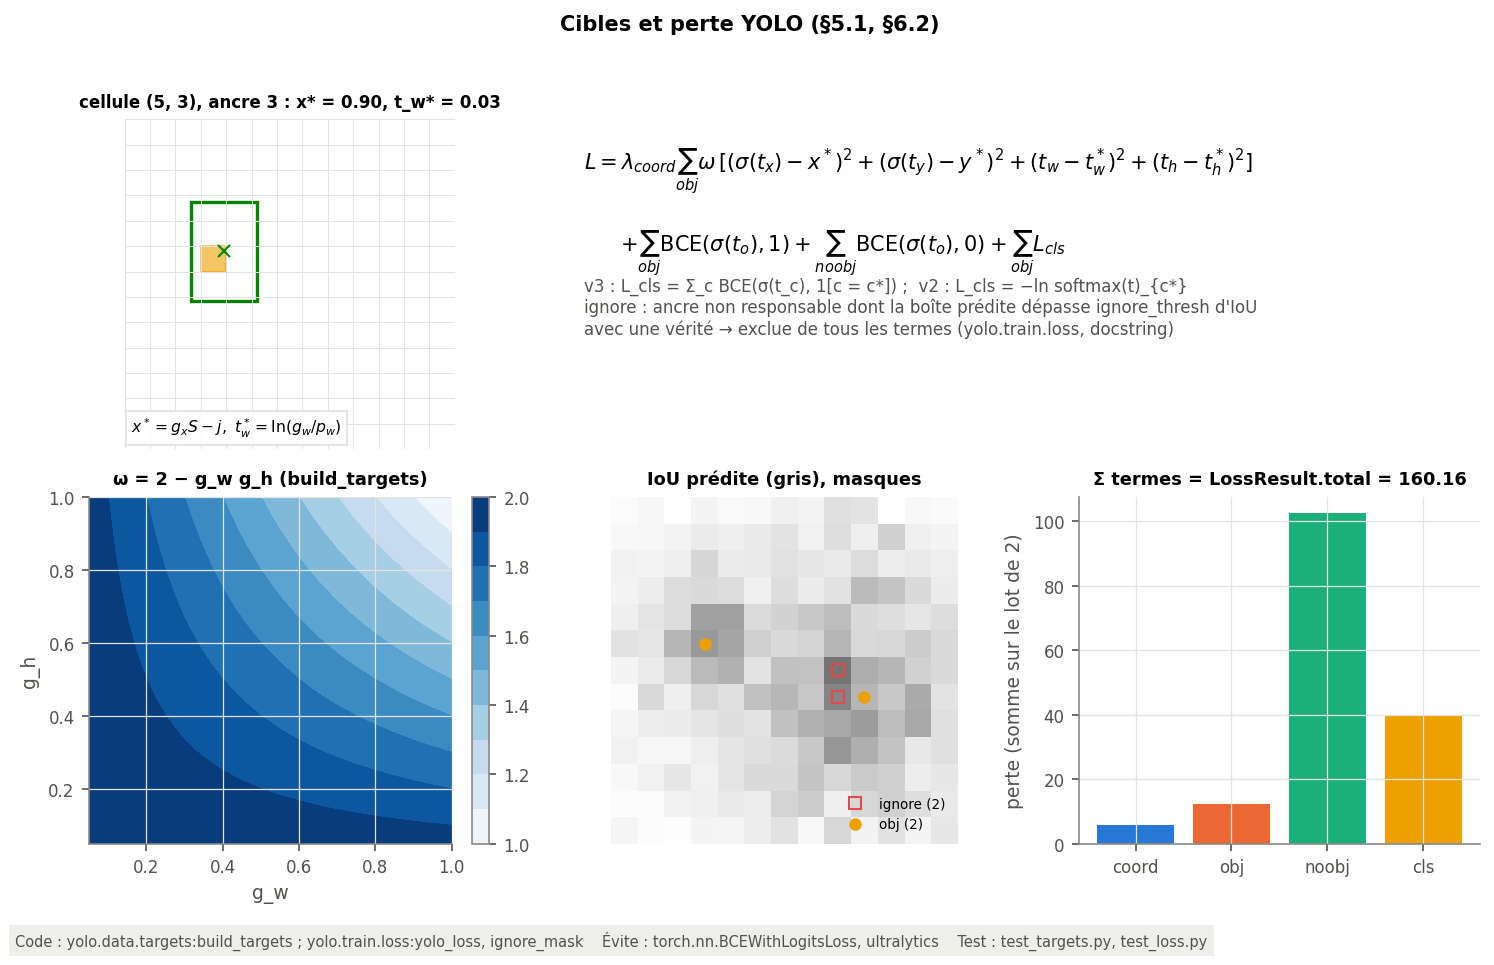
\includegraphics[width=\linewidth,height=0.42\textheight,keepaspectratio]{../../results/figures/maths/perte.png}
\caption{Cibles et perte YOLO : encodage d'une vérité, la perte terme par terme, le poids $\omega$ = 2 − g\_w g\_h, le masque ignore et la part de chaque terme sur un lot. (\texttt{perte})}
\label{fig:perte}
% python -m tools.figures perte
\end{figure}}
\expandafter\def\csname artfig:pr/pr_variantes\endcsname{%
\begin{figure}[htbp]
\centering
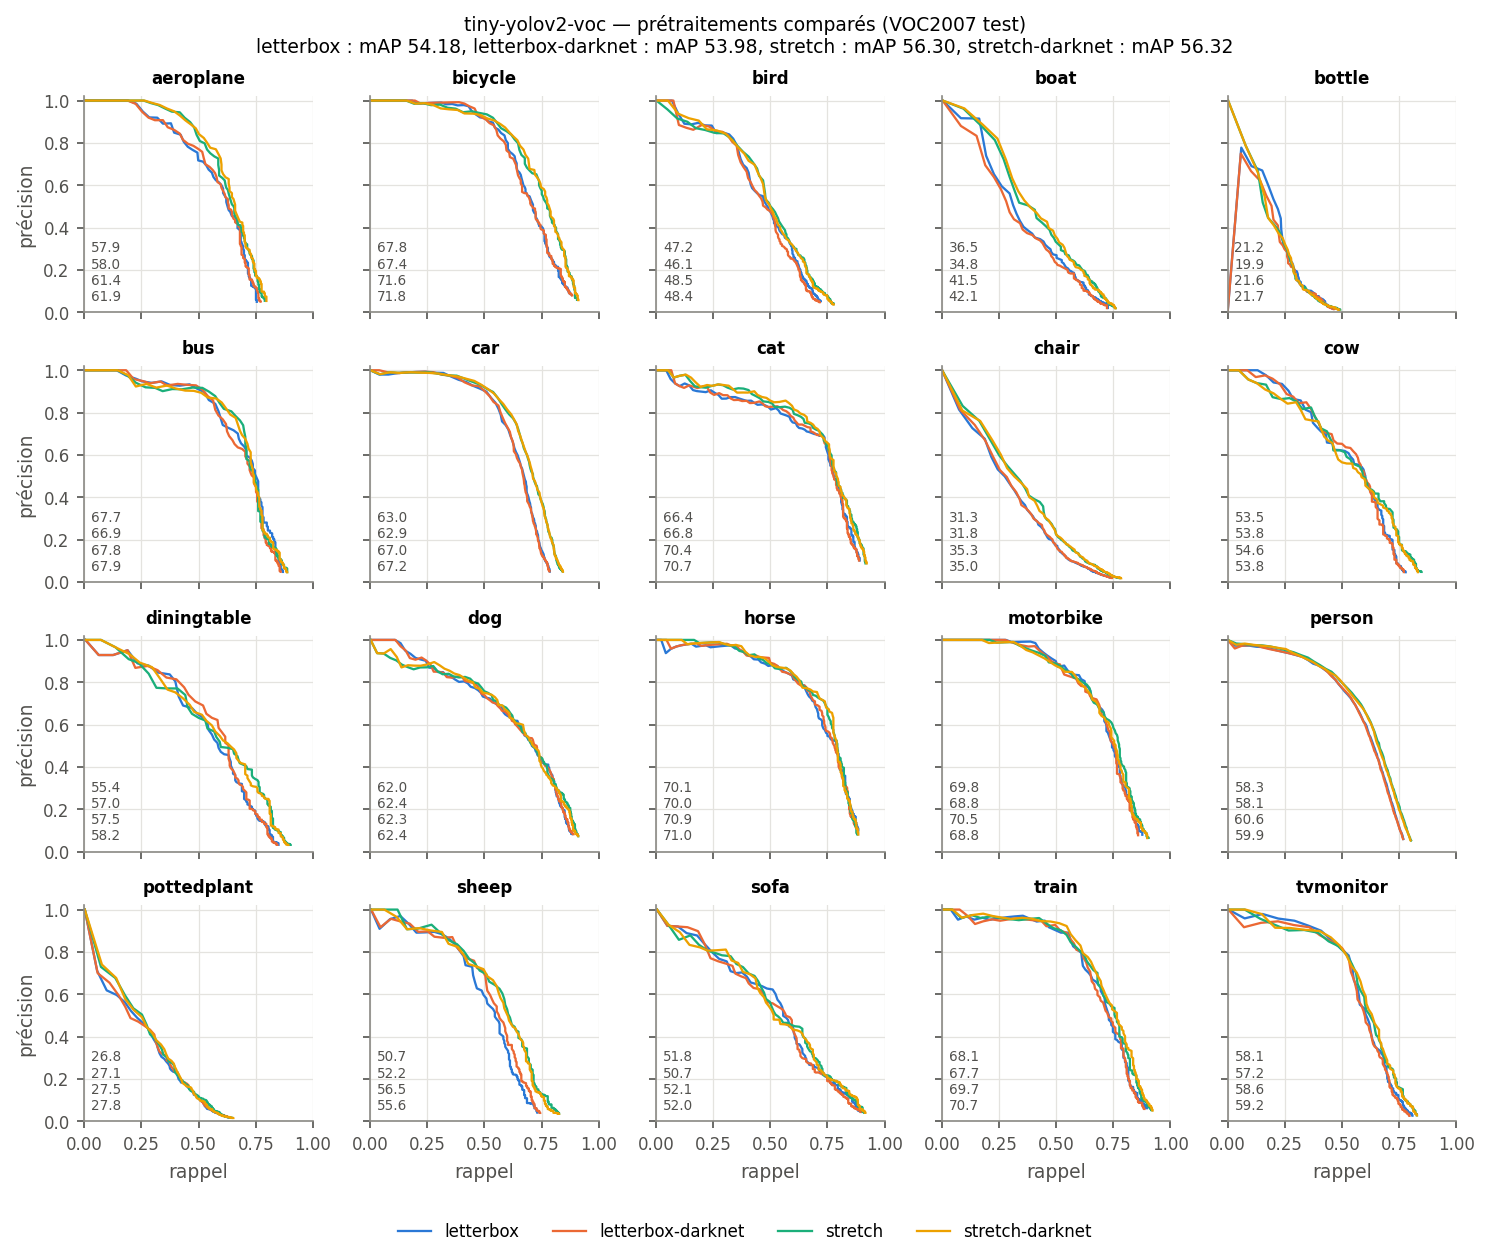
\includegraphics[width=\linewidth,height=0.42\textheight,keepaspectratio]{../../results/figures/resultats/pr_variantes.png}
\caption{Courbes précision-rappel par classe (11 points VOC07) pour chaque prétraitement évalué, puis les quatre superposées. (\texttt{pr})}
\label{fig:pr/pr_variantes}
% python -m tools.figures pr
\end{figure}}
\expandafter\def\csname artfig:nms_map\endcsname{%
\begin{figure}[htbp]
\centering
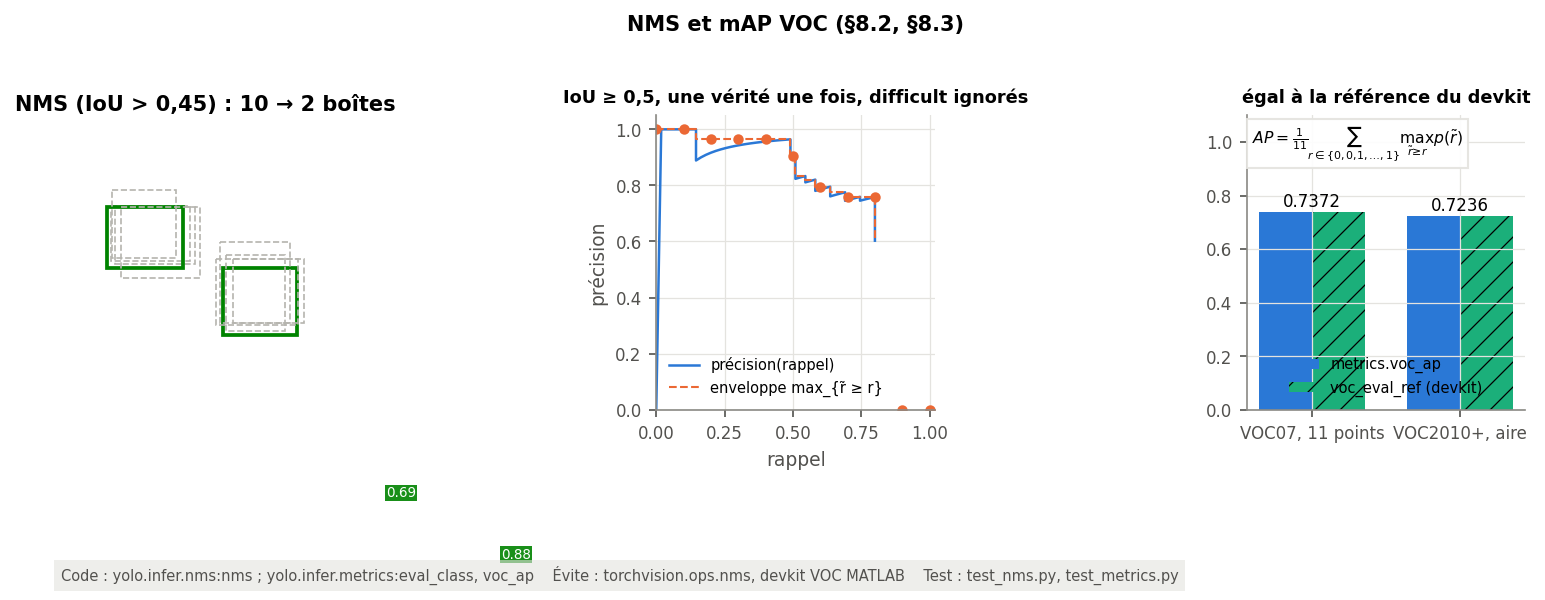
\includegraphics[width=\linewidth,height=0.42\textheight,keepaspectratio]{../../results/figures/maths/nms_map.png}
\caption{NMS pas à pas, appariement détections / vérités et courbe précision-rappel, AP VOC07 sur 11 points face à l'aire sous l'enveloppe, égale à la référence du devkit. (\texttt{nms\_map})}
\label{fig:nms_map}
% python -m tools.figures nms_map
\end{figure}}
\expandafter\def\csname artfig:quantification\endcsname{%
\begin{figure}[htbp]
\centering
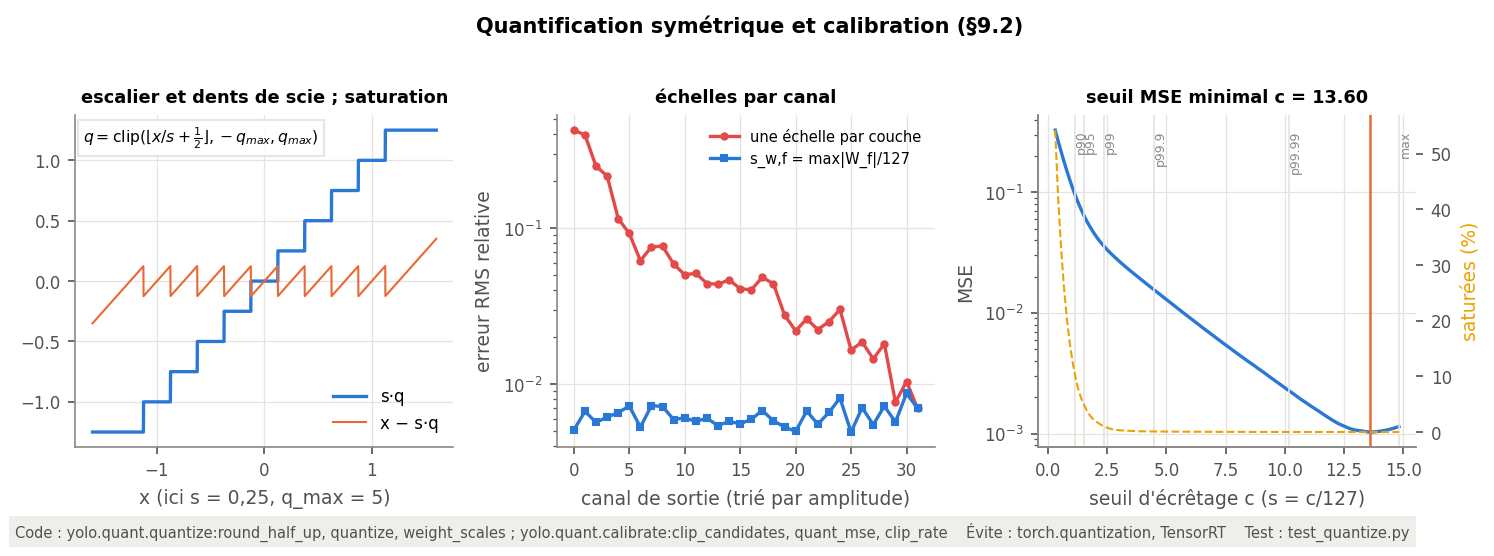
\includegraphics[width=\linewidth,height=0.42\textheight,keepaspectratio]{../../results/figures/maths/quantification.png}
\caption{Quantification symétrique : l'escalier et son erreur, échelles par canal face à une échelle par couche, choix du seuil d'écrêtage par la MSE. (\texttt{quantification})}
\label{fig:quantification}
% python -m tools.figures quantification
\end{figure}}
\expandafter\def\csname artfig:entier\endcsname{%
\begin{figure}[htbp]
\centering
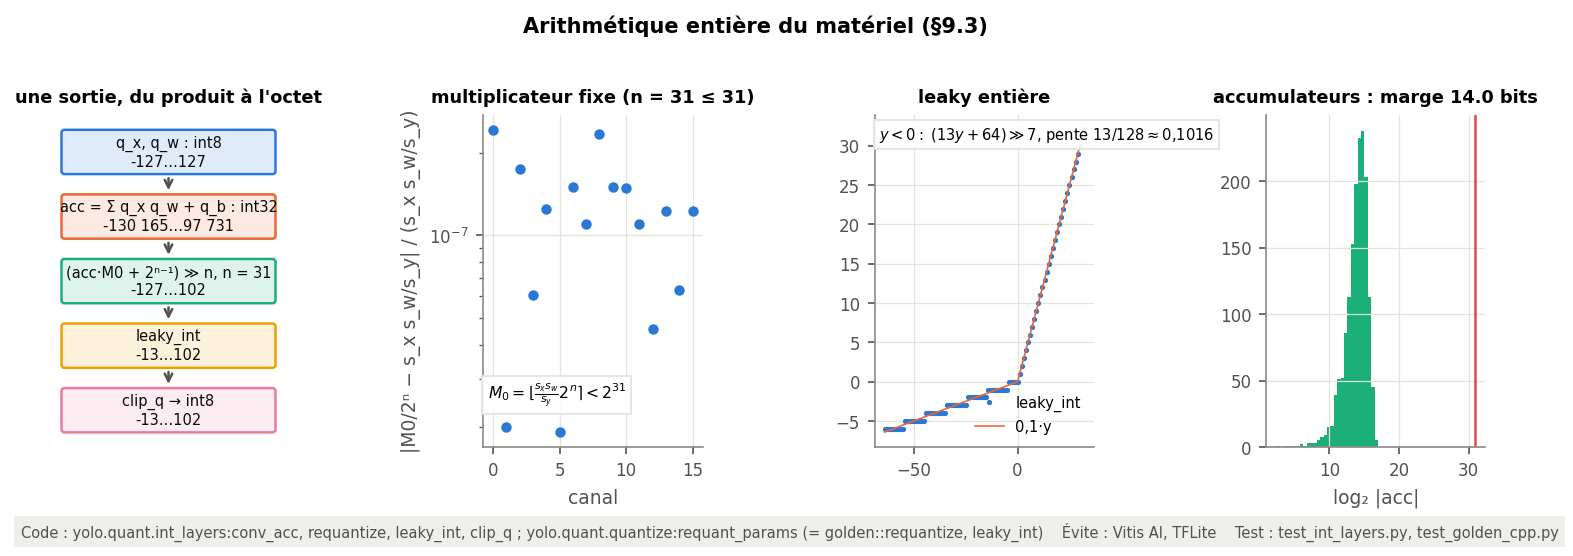
\includegraphics[width=\linewidth,height=0.42\textheight,keepaspectratio]{../../results/figures/maths/entier.png}
\caption{Arithmétique entière du matériel : chaîne d'une sortie, multiplicateur fixe M0/2$^n$, leaky entière 13/128 et marge des accumulateurs int32. (\texttt{entier})}
\label{fig:entier}
% python -m tools.figures entier
\end{figure}}
\expandafter\def\csname artfig:calibration/calibration_tiny-yolov2-voc\endcsname{%
\begin{figure}[htbp]
\centering
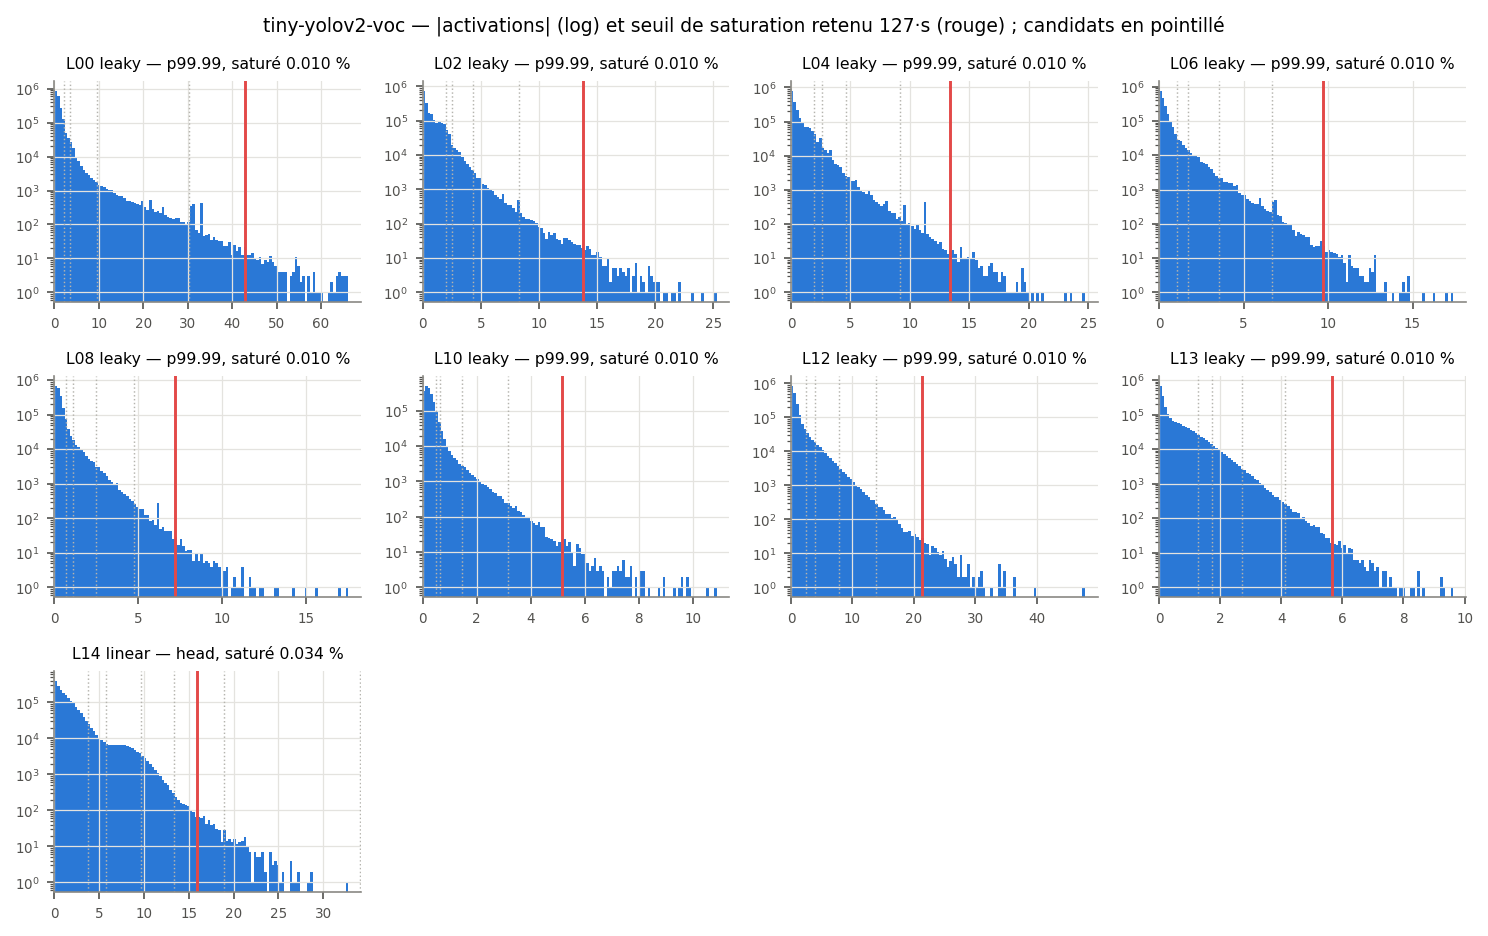
\includegraphics[width=\linewidth,height=0.42\textheight,keepaspectratio]{../../results/figures/resultats/calibration_tiny-yolov2-voc.png}
\caption{Distribution des activations par couche et seuil de saturation retenu par la calibration ; échelles des poids par canal. (\texttt{calibration})}
\label{fig:calibration/calibration_tiny-yolov2-voc}
% python -m tools.figures calibration
\end{figure}}
\expandafter\def\csname artfig:erreur_couches/erreur_couches_tiny-yolov2-voc\endcsname{%
\begin{figure}[htbp]
\centering
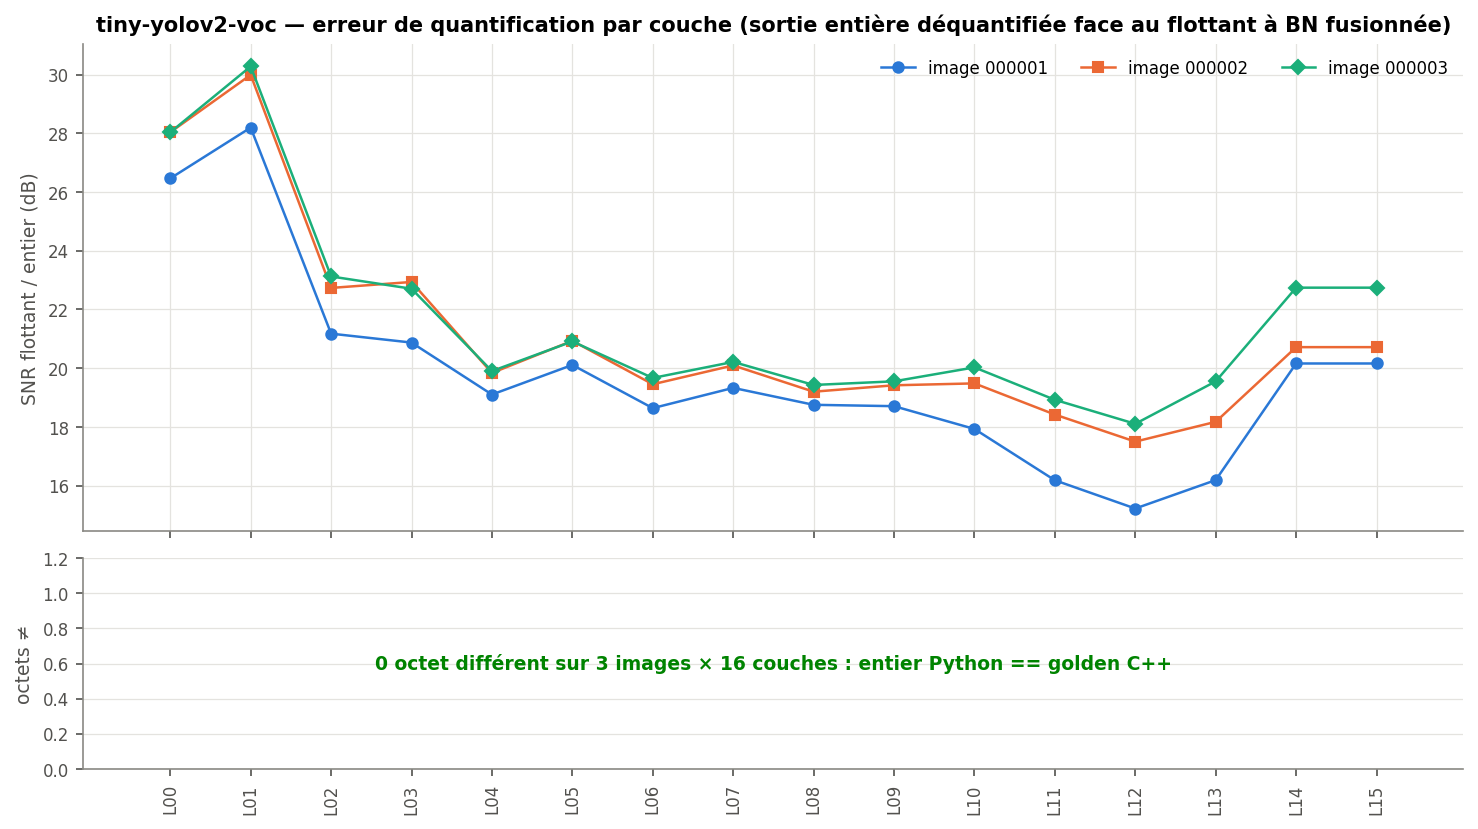
\includegraphics[width=\linewidth,height=0.42\textheight,keepaspectratio]{../../results/figures/resultats/erreur_couches_tiny-yolov2-voc.png}
\caption{SNR par couche entre le flottant et l'entier déquantifié, et écart entier Python $\leftrightarrow$ golden C++ (0 partout : bit-exact). (\texttt{erreur\_couches})}
\label{fig:erreur_couches/erreur_couches_tiny-yolov2-voc}
% python -m tools.figures erreur_couches
\end{figure}}
\expandafter\def\csname artfig:chaine_verif\endcsname{%
\begin{figure}[htbp]
\centering
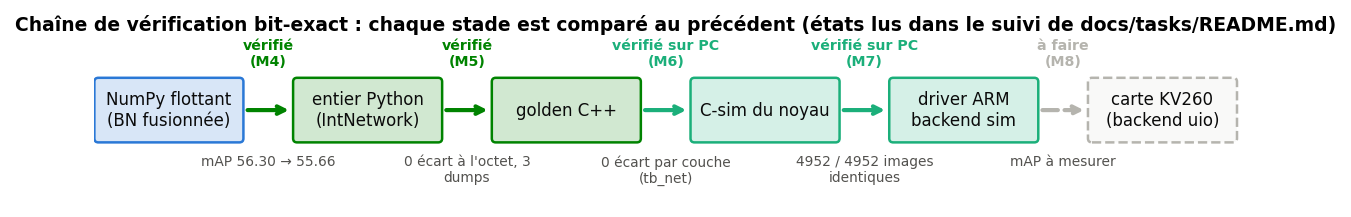
\includegraphics[width=\linewidth,height=0.42\textheight,keepaspectratio]{../../results/figures/materiel/chaine_verif.png}
\caption{Chaîne de vérification bit-exact, du flottant NumPy à la carte : critère et état de chaque passage. (\texttt{chaine\_verif})}
\label{fig:chaine_verif}
% python -m tools.figures chaine_verif
\end{figure}}
\expandafter\def\csname artfig:moteur\endcsname{%
\begin{figure}[htbp]
\centering
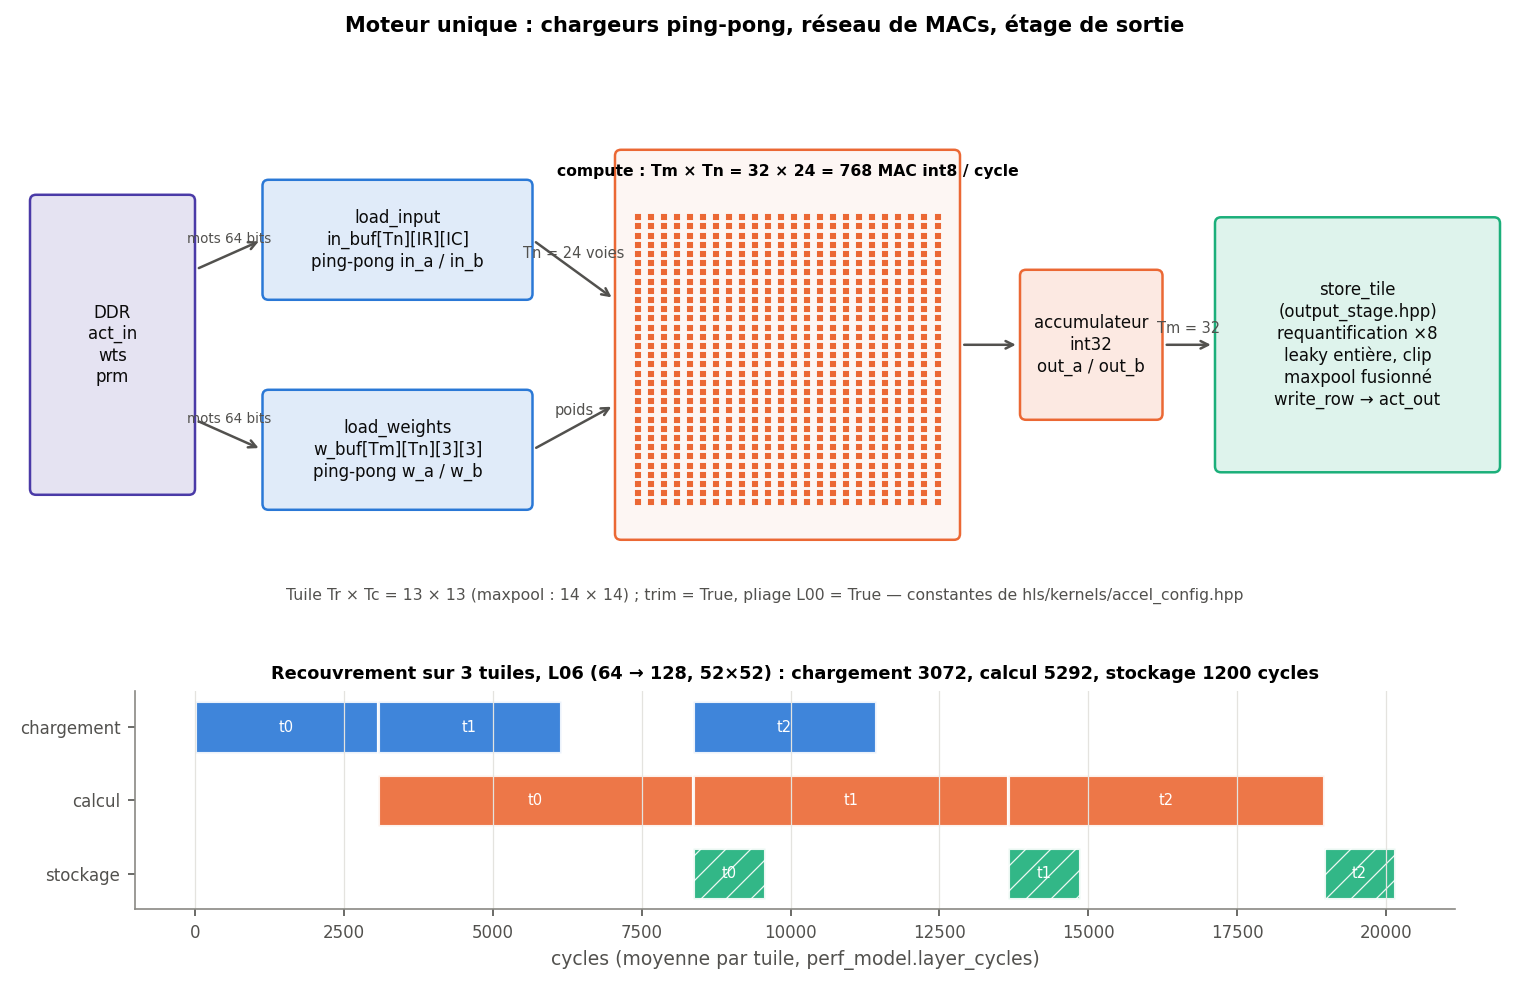
\includegraphics[width=\linewidth,height=0.42\textheight,keepaspectratio]{../../results/figures/materiel/moteur.png}
\caption{Moteur unique : chargeurs ping-pong, réseau Tm × Tn de MACs, accumulateur, étage de sortie, et chronogramme du recouvrement sur 3 tuiles. (\texttt{moteur})}
\label{fig:moteur}
% python -m tools.figures moteur
\end{figure}}
\expandafter\def\csname artfig:tuilage\endcsname{%
\begin{figure}[htbp]
\centering
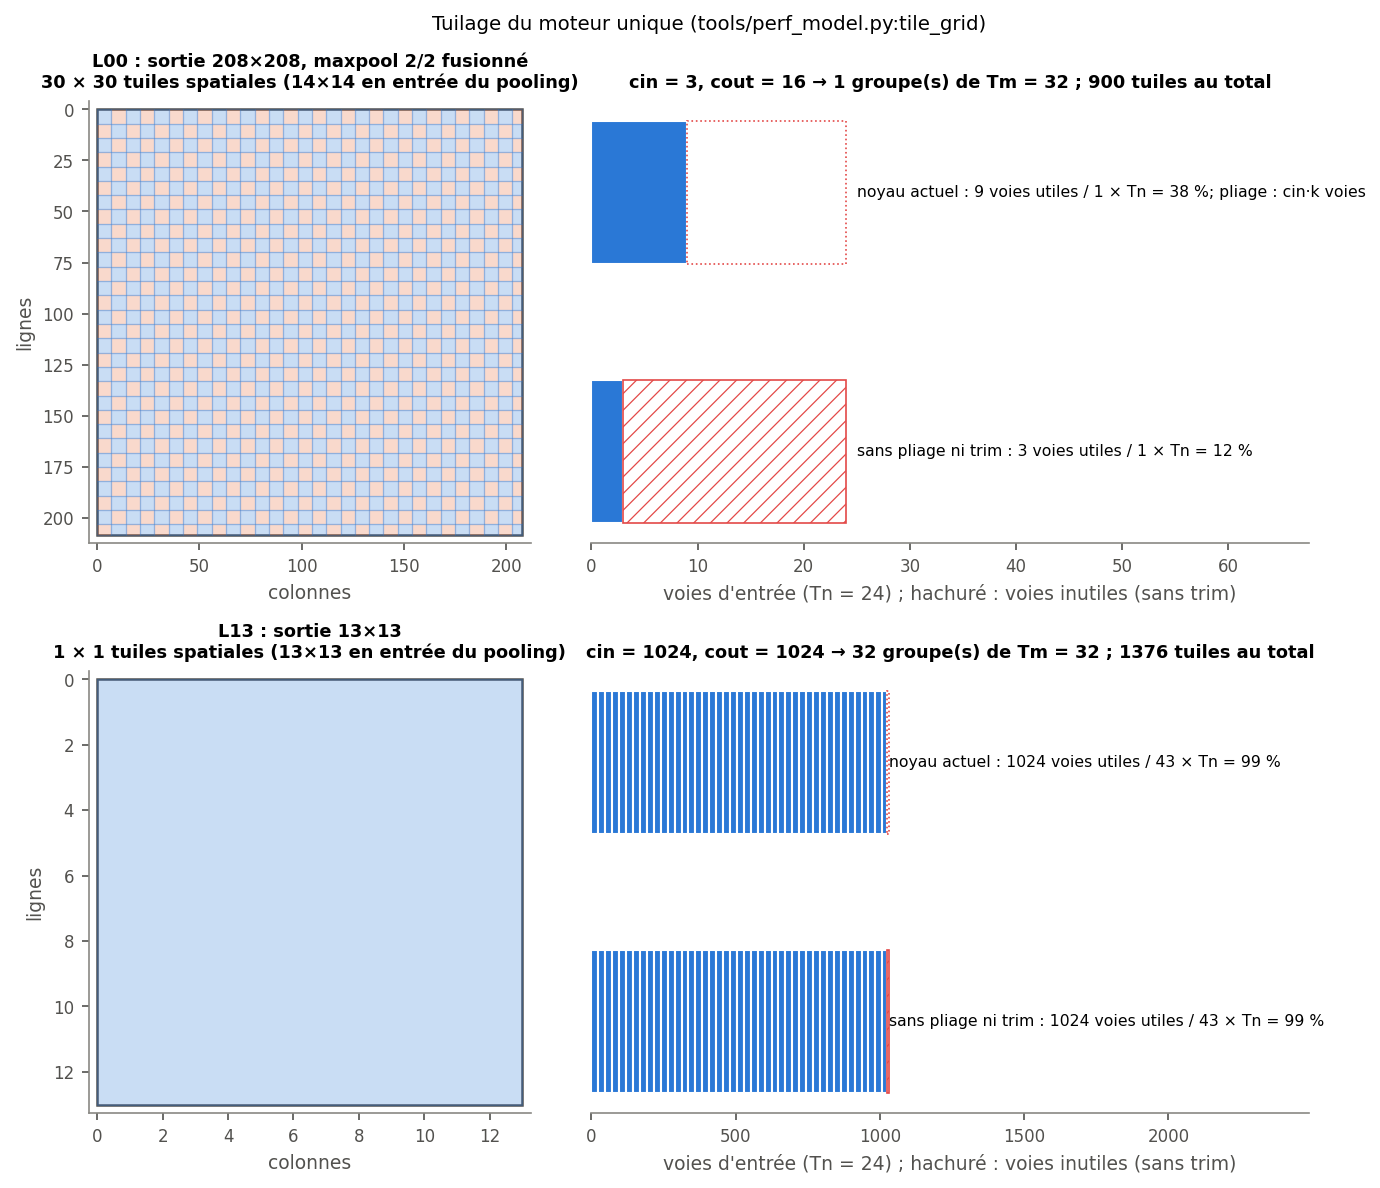
\includegraphics[width=\linewidth,height=0.42\textheight,keepaspectratio]{../../results/figures/materiel/tuilage.png}
\caption{Tuilage de deux couches : tuiles spatiales et voies d'entrée, avec le pliage de L00 (cin = 3) et la couche 13×13 couverte par une seule tuile. (\texttt{tuilage})}
\label{fig:tuilage}
% python -m tools.figures tuilage
\end{figure}}
\expandafter\def\csname artfig:soc\endcsname{%
\begin{figure}[htbp]
\centering
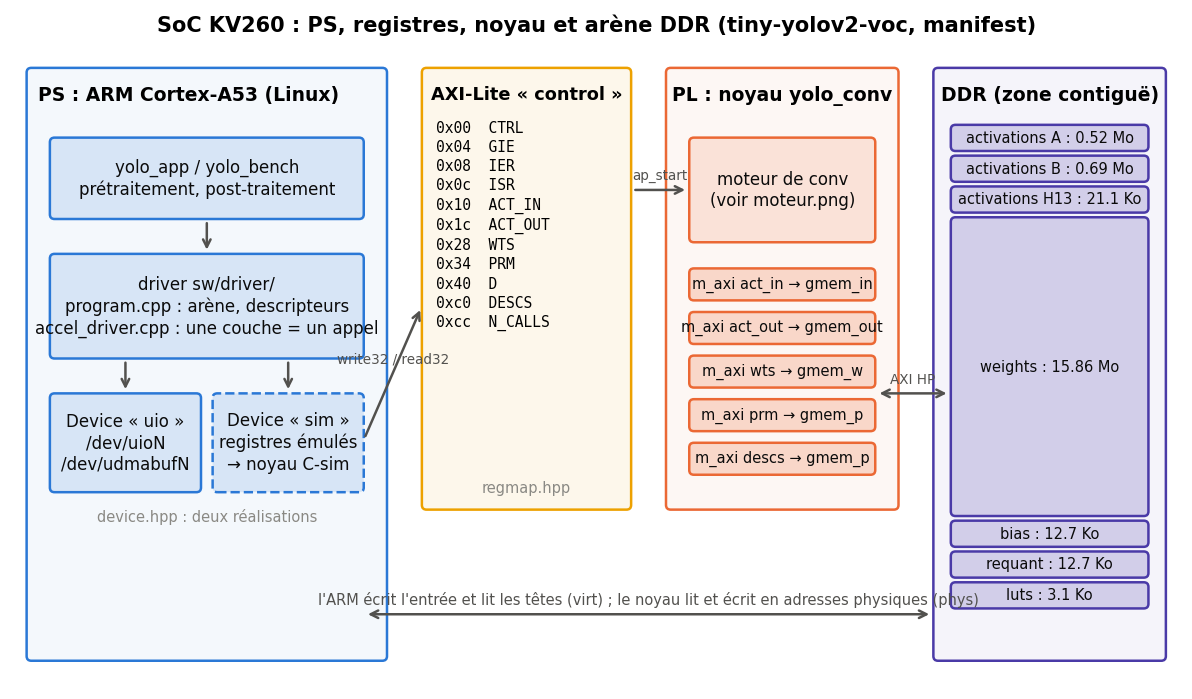
\includegraphics[width=\linewidth,height=0.42\textheight,keepaspectratio]{../../results/figures/materiel/soc.png}
\caption{Schéma du SoC : application et driver sur l'ARM, registres AXI-Lite, ports m\_axi du noyau et découpage de l'arène DDR. (\texttt{soc})}
\label{fig:soc}
% python -m tools.figures soc
\end{figure}}
\expandafter\def\csname artfig:cascade_m10\endcsname{%
\begin{figure}[htbp]
\centering
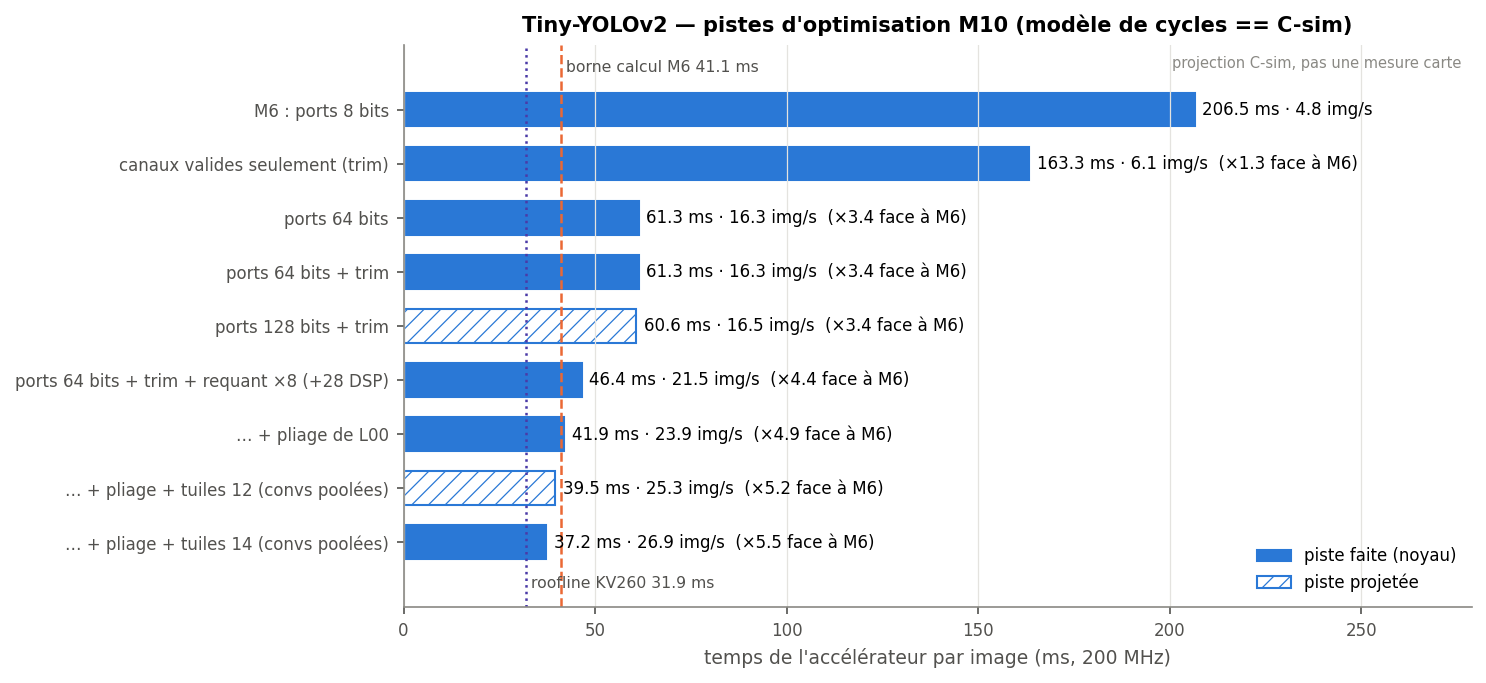
\includegraphics[width=\linewidth,height=0.42\textheight,keepaspectratio]{../../results/figures/resultats/cascade_m10.png}
\caption{Temps par image de Tiny-YOLOv2 à chaque piste d'optimisation M10, face à la borne de calcul et au roofline KV260. (\texttt{cascade\_m10})}
\label{fig:cascade_m10}
% python -m tools.figures cascade_m10
\end{figure}}
\expandafter\def\csname artfig:roofline_couches/roofline_couches_kv260\endcsname{%
\begin{figure}[htbp]
\centering
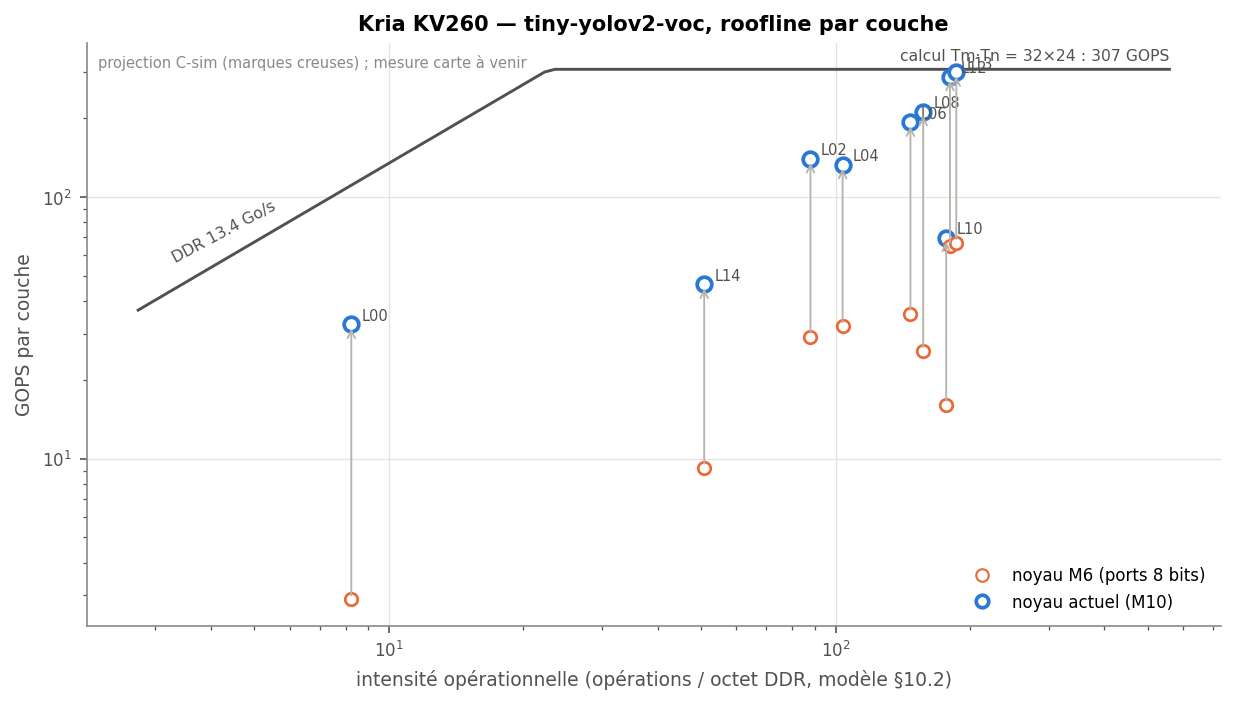
\includegraphics[width=\linewidth,height=0.42\textheight,keepaspectratio]{../../results/figures/resultats/roofline_couches_kv260.png}
\caption{Roofline KV260 avec un point par couche de Tiny-YOLOv2, avant et après les optimisations M10. (\texttt{roofline\_couches})}
\label{fig:roofline_couches/roofline_couches_kv260}
% python -m tools.figures roofline_couches
\end{figure}}
\expandafter\def\csname artfig:cycles_couches\endcsname{%
\begin{figure}[htbp]
\centering
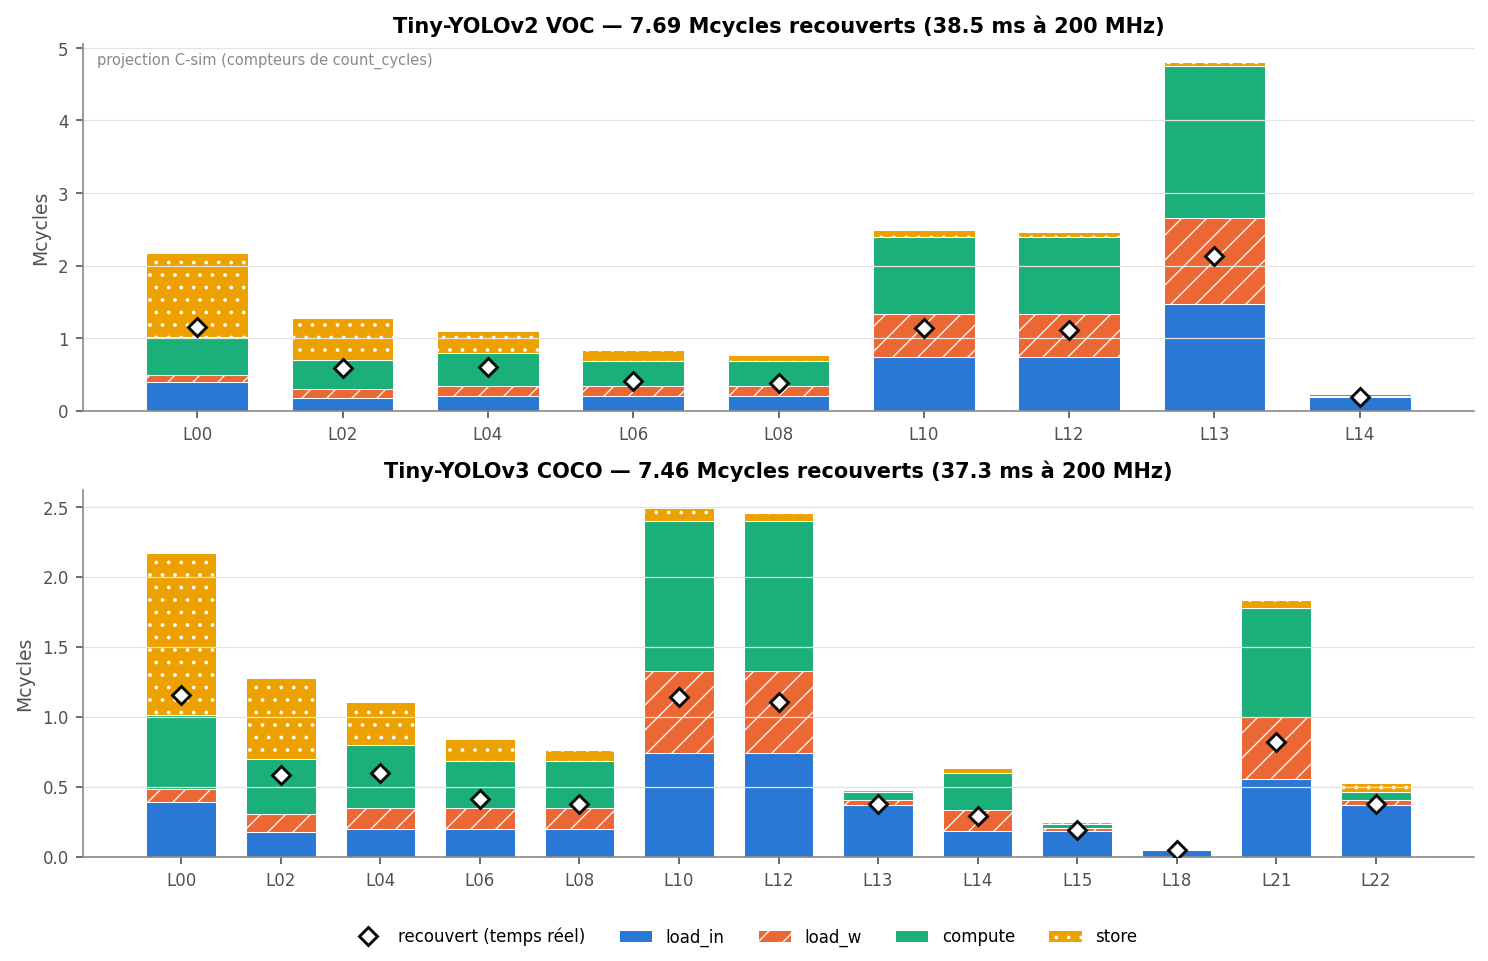
\includegraphics[width=\linewidth,height=0.42\textheight,keepaspectratio]{../../results/figures/resultats/cycles_couches.png}
\caption{Cycles par couche du noyau actuel, décomposés en chargements, calcul et stockage ; le losange donne le temps réel avec recouvrement. (\texttt{cycles\_couches})}
\label{fig:cycles_couches}
% python -m tools.figures cycles_couches
\end{figure}}
\expandafter\def\csname artfig:map_stades\endcsname{%
\begin{figure}[htbp]
\centering
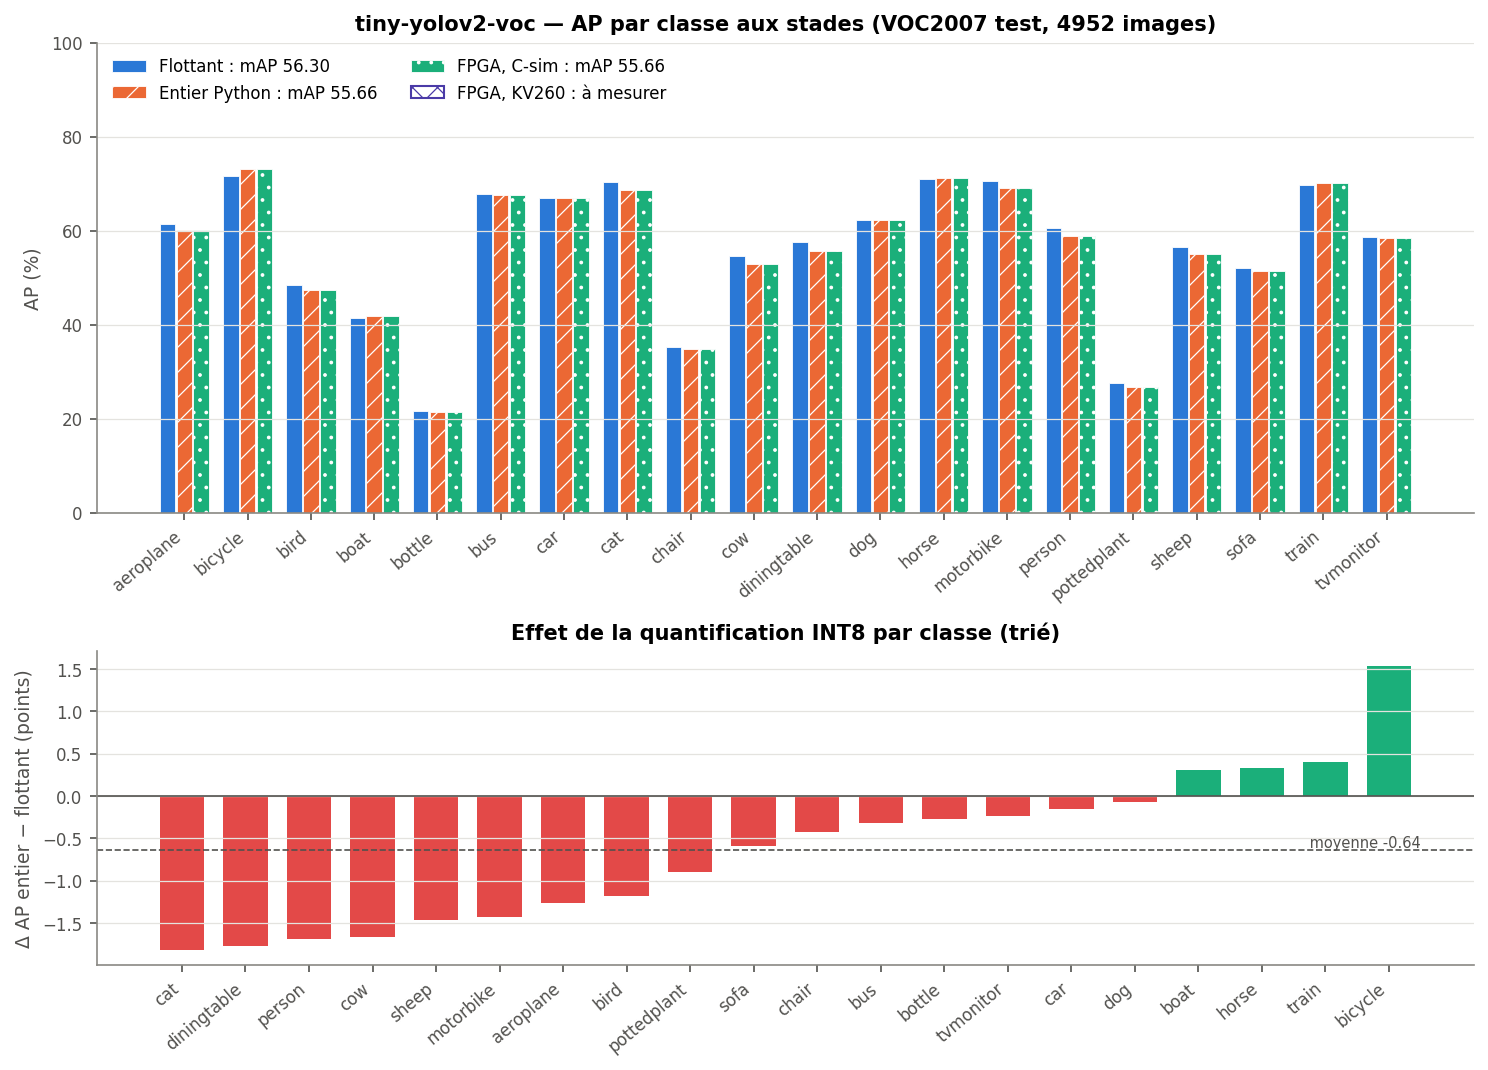
\includegraphics[width=\linewidth,height=0.42\textheight,keepaspectratio]{../../results/figures/resultats/map_stades.png}
\caption{AP par classe aux stades flottant, entier et C-sim (la carte quand elle sera mesurée), et écart entier − flottant trié. (\texttt{map\_stades})}
\label{fig:map_stades}
% python -m tools.figures map_stades
\end{figure}}
\expandafter\def\csname artfig:ressources\endcsname{%
\begin{figure}[htbp]
\centering
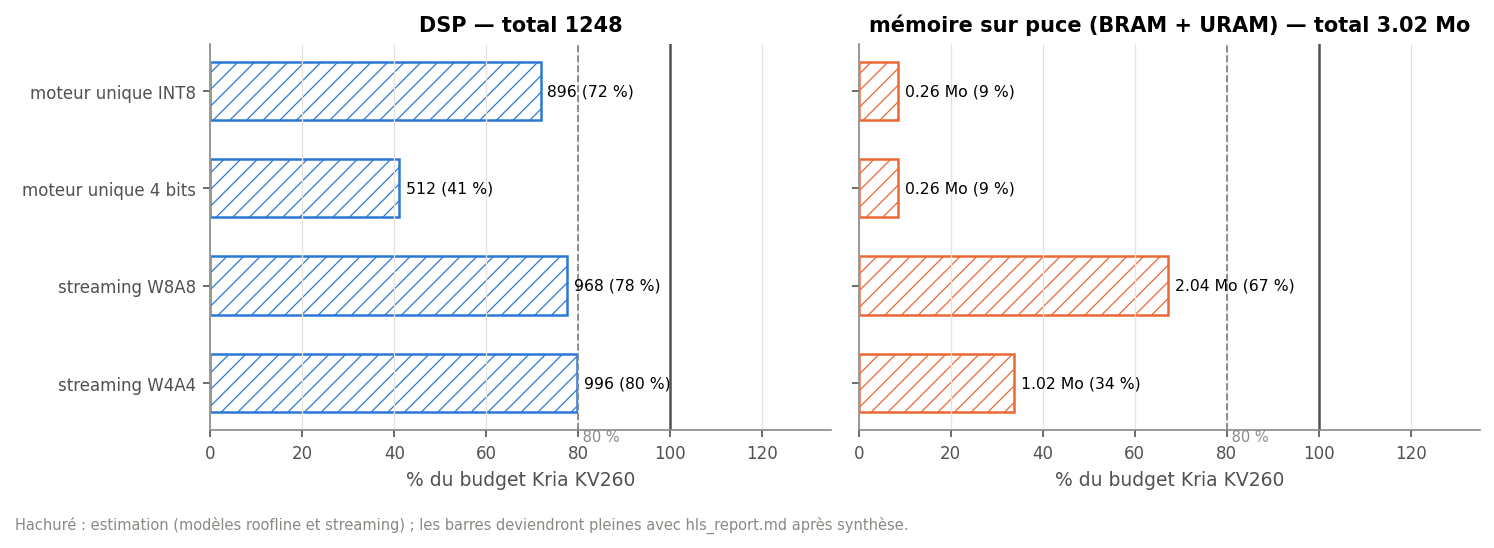
\includegraphics[width=\linewidth,height=0.42\textheight,keepaspectratio]{../../results/figures/resultats/ressources.png}
\caption{DSP, mémoire sur puce et LUT des architectures (moteur unique INT8, pow2 et 4 bits, streaming) face au budget de la KV260 ; hachuré : estimation, plein : synthèse. (\texttt{ressources})}
\label{fig:ressources}
% python -m tools.figures ressources
\end{figure}}
\expandafter\def\csname artfig:hw_postproc\endcsname{%
\begin{figure}[htbp]
\centering
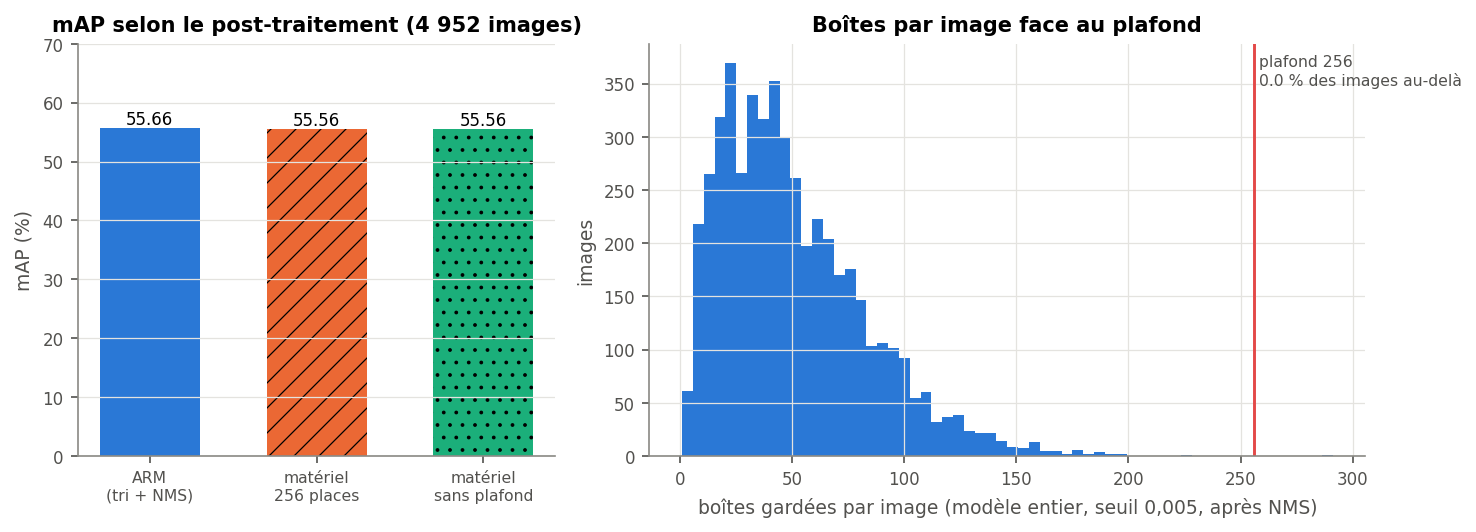
\includegraphics[width=\linewidth,height=0.42\textheight,keepaspectratio]{../../results/figures/resultats/hw_postproc.png}
\caption{mAP avec le post-traitement matériel, avec et sans plafond de boîtes, et nombre de boîtes par image face au plafond. (\texttt{hw\_postproc})}
\label{fig:hw_postproc}
% python -m tools.figures hw_postproc
\end{figure}}
\expandafter\def\csname artfig:map_formats\endcsname{%
\begin{figure}[htbp]
\centering
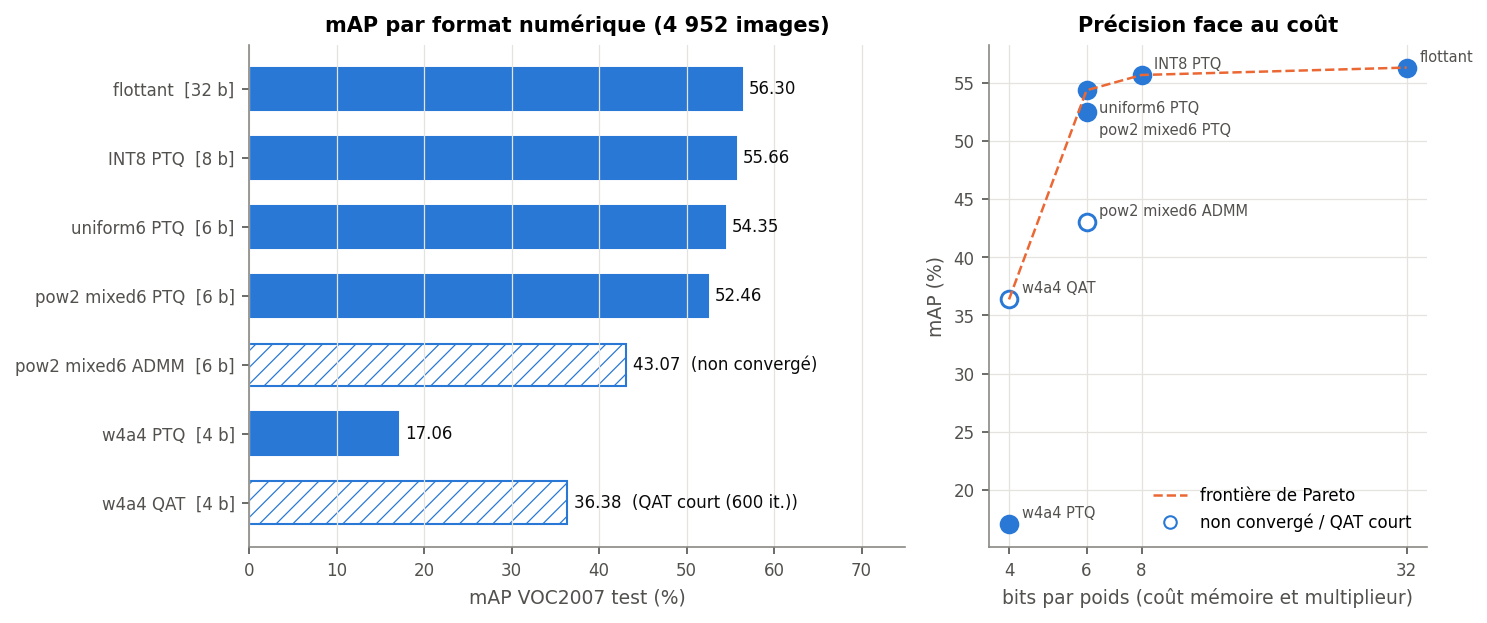
\includegraphics[width=\linewidth,height=0.42\textheight,keepaspectratio]{../../results/figures/resultats/map_formats.png}
\caption{mAP de Tiny-YOLOv2 selon le format des poids (flottant, INT8, puissances de 2, 4 bits), et frontière précision / bits. (\texttt{map\_formats})}
\label{fig:map_formats}
% python -m tools.figures map_formats
\end{figure}}
\expandafter\def\csname artfig:streaming\endcsname{%
\begin{figure}[htbp]
\centering
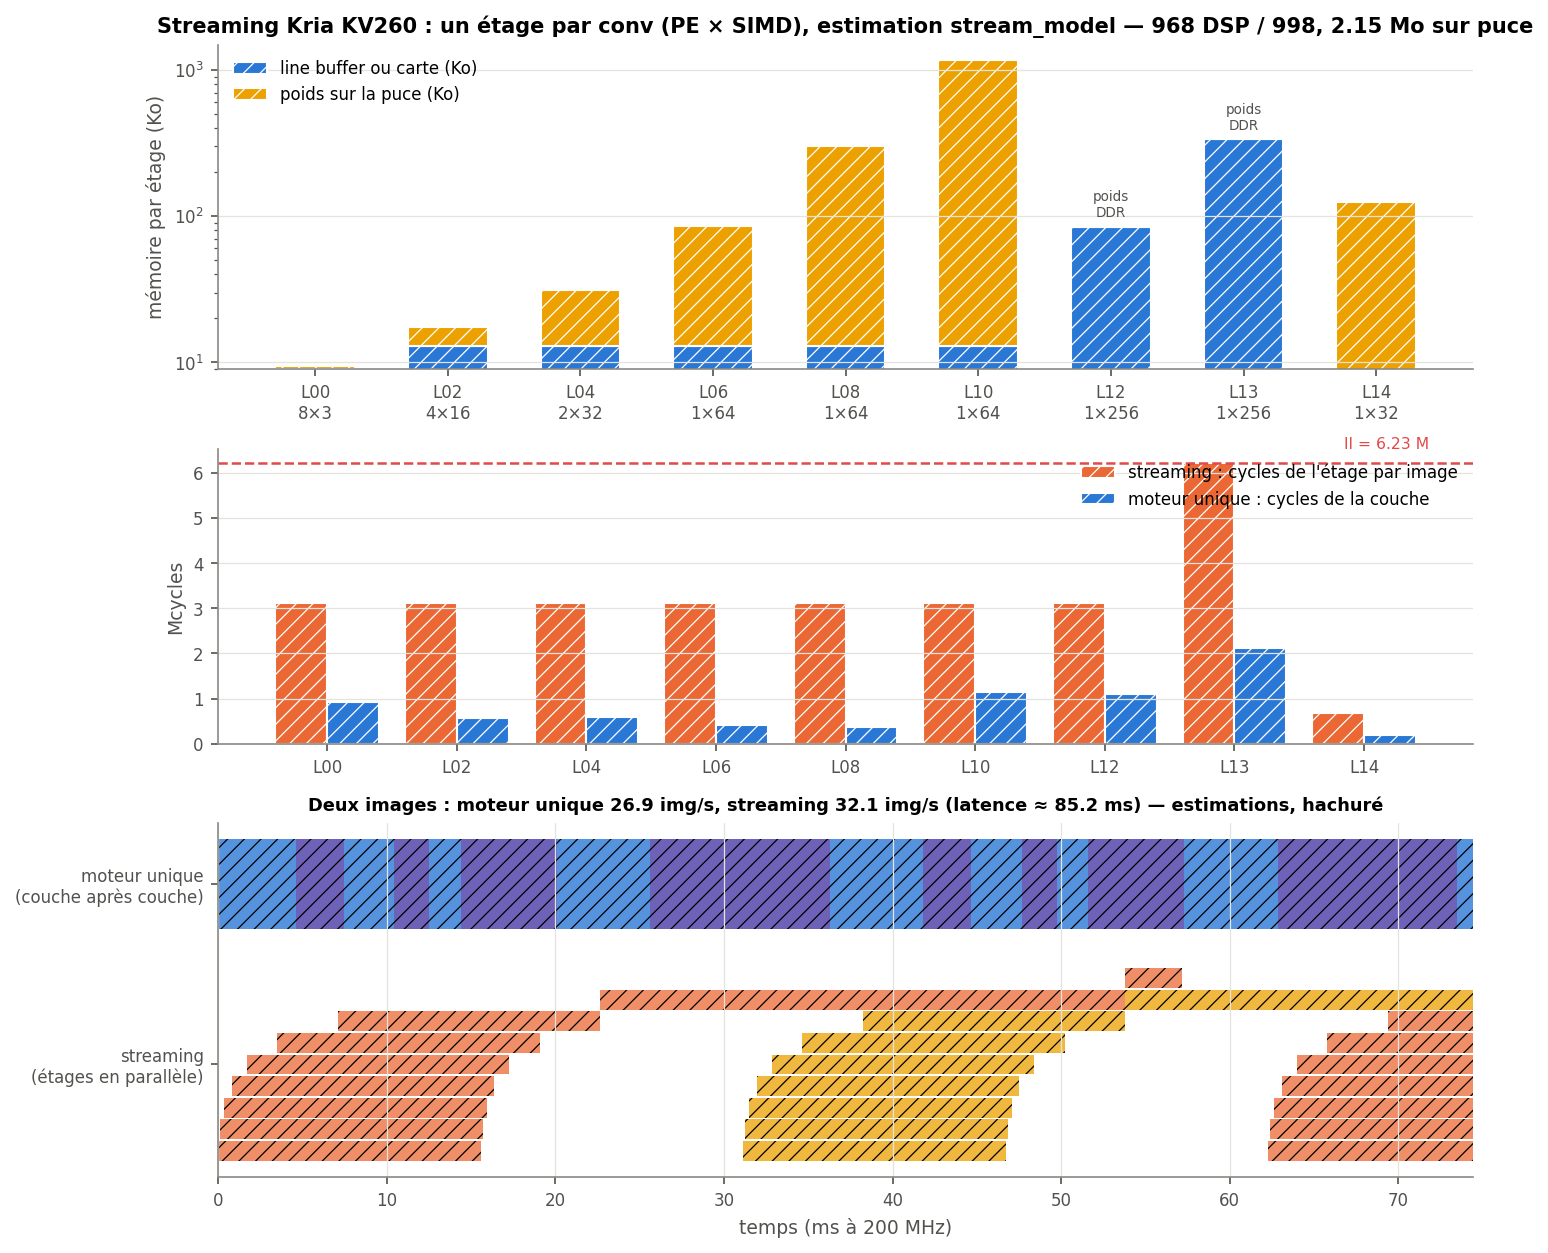
\includegraphics[width=\linewidth,height=0.42\textheight,keepaspectratio]{../../results/figures/materiel/streaming.png}
\caption{Architecture streaming face au moteur unique : mémoire et parallélisme par étage, cycles par couche, chronogramme sur deux images (estimations). (\texttt{streaming})}
\label{fig:streaming}
% python -m tools.figures streaming
\end{figure}}
\expandafter\def\csname artfig:detections\endcsname{%
\begin{figure}[htbp]
\centering
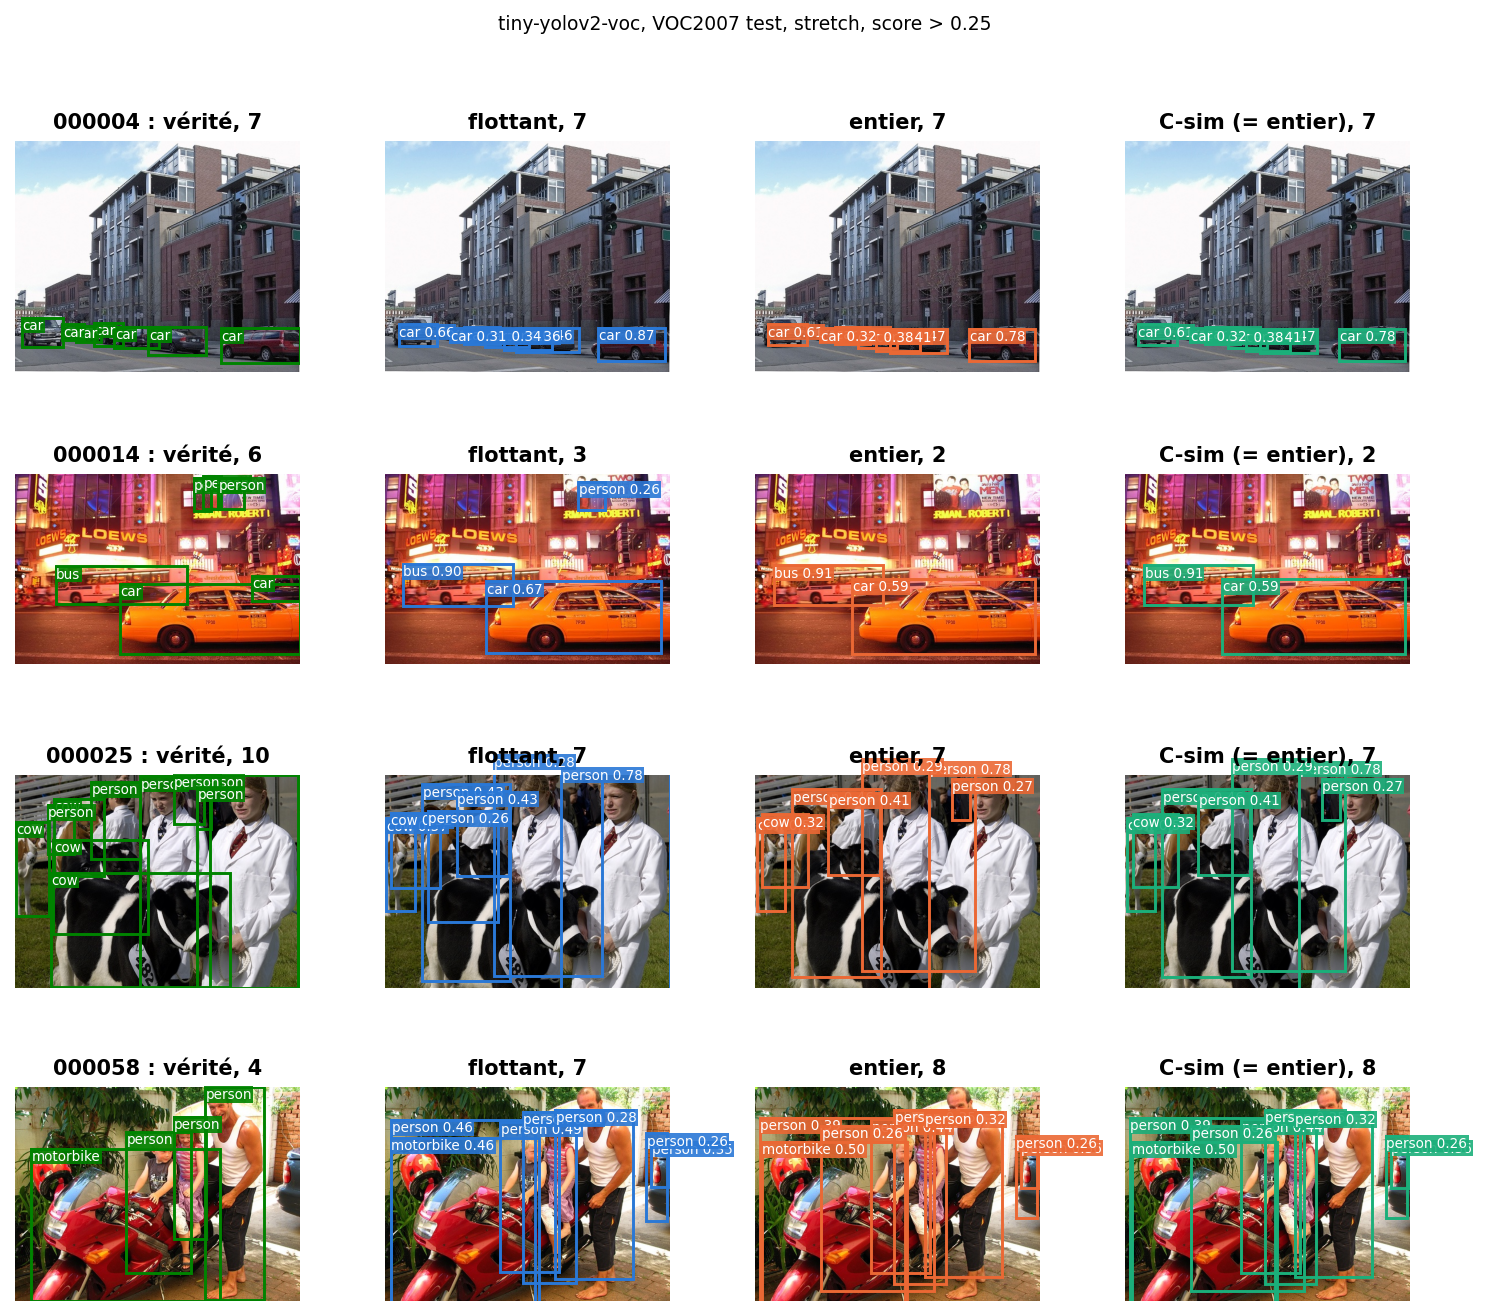
\includegraphics[width=\linewidth,height=0.42\textheight,keepaspectratio]{../../results/figures/resultats/detections.png}
\caption{Vérité terrain, flottant, entier et C-sim sur quatre images de VOC2007 test : les colonnes entier et C-sim sont identiques. (\texttt{detections})}
\label{fig:detections}
% python -m tools.figures detections
\end{figure}}
\expandafter\def\csname artfig:tests\endcsname{%
\begin{figure}[htbp]
\centering
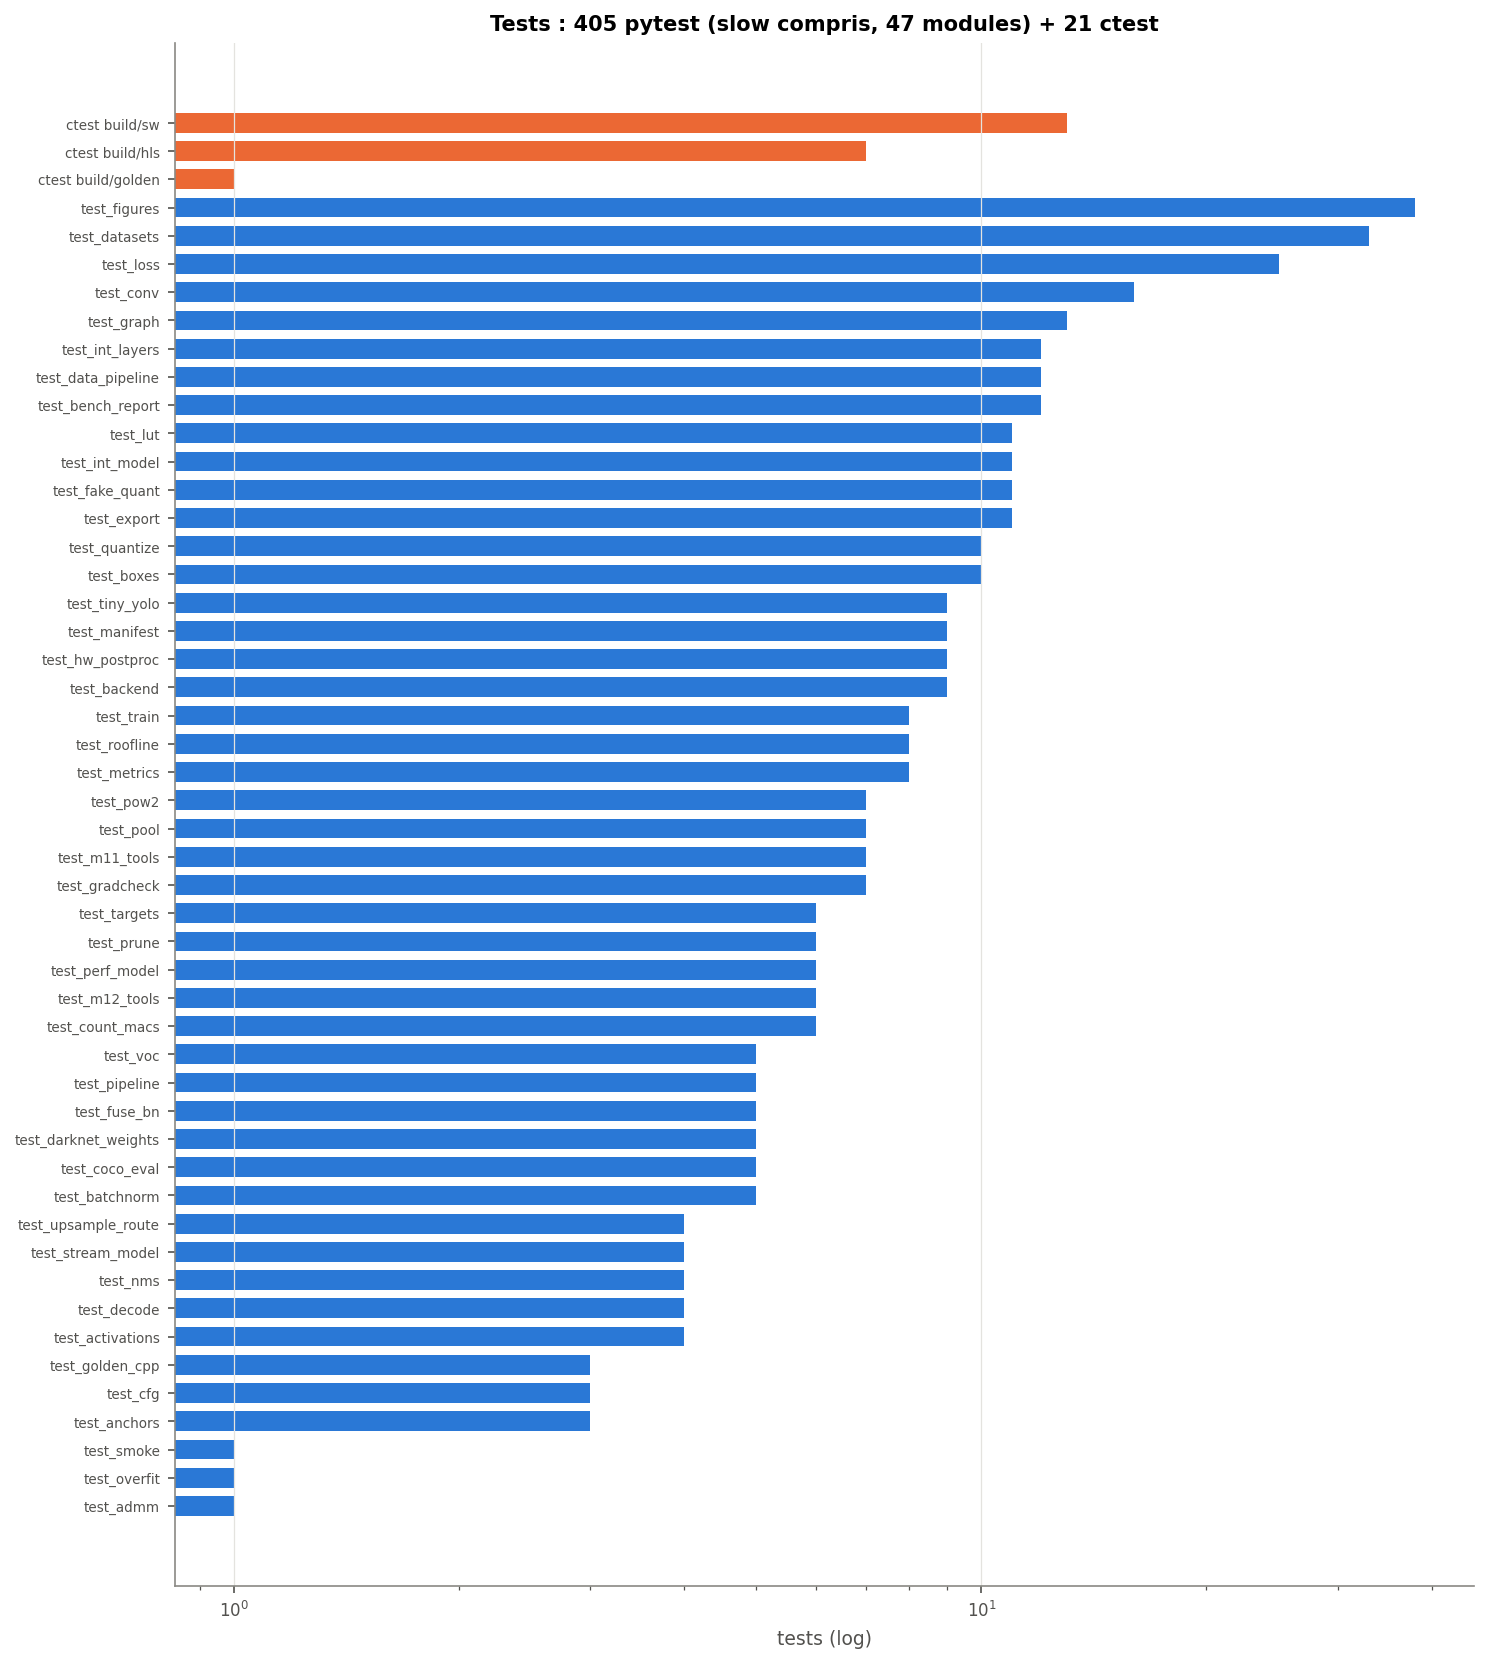
\includegraphics[width=\linewidth,height=0.42\textheight,keepaspectratio]{../../results/figures/projet/tests.png}
\caption{Nombre de tests par module Python (pytest, slow compris) et par build C++ (ctest), et leur durée quand \texttt{make test-durations} a été lancé. (\texttt{tests})}
\label{fig:tests}
% python -m tools.figures tests
\end{figure}}
\expandafter\def\csname artfig:code\endcsname{%
\begin{figure}[htbp]
\centering
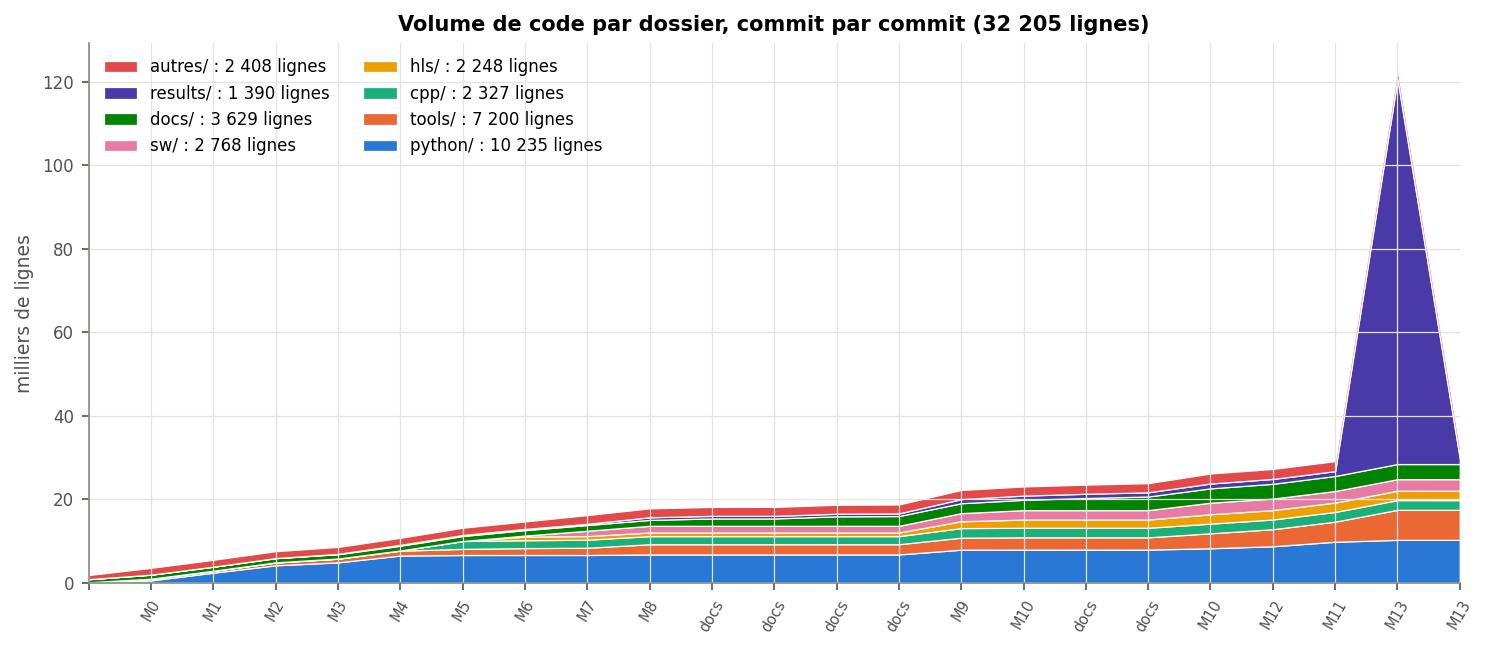
\includegraphics[width=\linewidth,height=0.42\textheight,keepaspectratio]{../../results/figures/projet/code.png}
\caption{Lignes par dossier (python, tools, cpp, hls, sw, docs, results) commit par commit. (\texttt{code})}
\label{fig:code}
% python -m tools.figures code
\end{figure}}
% ---- milestones, pending keys, revision
\newcommand\articleetat{%
\begin{tabular}{@{}lrrr@{}}
\toprule
\textbf{Milestone} & \textbf{Tasks} & \textbf{Done} & \textbf{Progress} \\
\midrule
M0 & 6 & 6 & 100\,\% \\
M1 & 9 & 8 & 89\,\% \\
M2 & 9 & 8 & 89\,\% \\
M3 & 4 & 4 & 100\,\% \\
M4 & 7 & 7 & 100\,\% \\
M5 & 6 & 6 & 100\,\% \\
M6 & 6 & 1 & 17\,\% \\
M7 & 4 & 0 & 0\,\% \\
M8 & 3 & 0 & 0\,\% \\
M9 & 1 & 0 & 0\,\% \\
M9.1 & 3 & 2 & 67\,\% \\
M9.2 & 4 & 3 & 75\,\% \\
M9.3 & 5 & 5 & 100\,\% \\
M9.4 & 3 & 3 & 100\,\% \\
M10 & 13 & 0 & 0\,\% \\
M12 & 11 & 0 & 0\,\% \\
M11 & 8 & 0 & 0\,\% \\
M13 & 54 & 54 & 100\,\% \\
M14 & 12 & 5 & 42\,\% \\
M15 & 16 & 1 & 6\,\% \\
M16 & 19 & 17 & 89\,\% \\
M17 & 21 & 17 & 81\,\% \\
M18 & 11 & 8 & 73\,\% \\
M19 & 12 & 0 & 0\,\% \\
\midrule
\textbf{Total} & \textbf{247} & \textbf{155} & \textbf{63\,\%} \\
\bottomrule
\end{tabular}}
\newcommand\articleetatresume{155 of 247 tasks done across 24 milestones, 7 milestones complete}
\newcommand\articlestatuslist{%
{\raggedright
\begin{itemize}
\item \textbf{projection} (10): \texttt{perf.cascade}, \texttt{perf.kv260}, \texttt{perf.kv260.bound.ms}, \texttt{perf.kv260.m6.ms}, \texttt{perf.kv260.roofline.ms}, \texttt{perf.kv260.v2.eff}, \texttt{perf.kv260.v2.fps}, \texttt{perf.kv260.v2.gops}, \texttt{perf.kv260.v2.ms}, \texttt{perf.kv260.v3.ms}
\item \textbf{estimate} (4): \texttt{stream.w4.fps}, \texttt{stream.w8.dsp}, \texttt{stream.w8.fps}, \texttt{stream.w8.latency}
\item \textbf{tier-R} (9): \texttt{balayage.crowdhuman.meilleur.map}, \texttt{balayage.exdark.meilleur.map}, \texttt{balayage.flir.meilleur.map}, \texttt{balayage.kitti.meilleur.map}, \texttt{balayage.visdrone.meilleur.map}, \texttt{balayage.voc.meilleur.map}, \texttt{balayages.meilleurs}, \texttt{quant.sensitive.gap}, \texttt{quant.sensitive.layer}
\item \textbf{csim} (3): \texttt{map.voc.csim}, \texttt{map.voc.identical}, \texttt{verif.hwpp.cases}
\end{itemize}\par}}
\newcommand\articlerev{rev.~\texttt{07c97e1-dirty}, 2026-10-07}


\title{Tiny-YOLO from scratch to an FPGA:\\a bit-exact chain from NumPy to an HLS
accelerator driven by an ARM SoC}
\author{Léonard Rivals}
\date{Draft, \articlerev}

\begin{document}
\maketitle

\begin{abstract}
We rewrite the Tiny-YOLOv2 and Tiny-YOLOv3 detectors from scratch in NumPy, without any
deep-learning library, with forward and backward passes checked by finite differences.
With the published Darknet weights, the float model reaches \chiffre{map.voc.float} mAP on
VOC2007 test (\chiffre{map.voc.images} images). We fuse batch normalization, quantize
weights per channel and activations per layer to INT8, and run the network in integer
arithmetic only: the gap to the float model is \chiffre{map.voc.drop} point
(\chiffre{map.voc.int8} mAP), without quantization-aware training. A C++ golden model and
a single-engine Vitis HLS accelerator reproduce the integer model byte for byte; driven by
the ARM driver over the C-simulated kernel, the whole test set gives
\chiffre{map.voc.identical} identical images, hence \chiffre{map.voc.csim} mAP. On a Kria
KV260 at 200~MHz, the cycle model of the optimized kernel projects
\chiffre{perf.kv260.v2.ms}~ms per image, i.e.\ \chiffre{perf.kv260.v2.gops} GOPS for
\chiffre{model.v2.gmacs} GMAC; the board itself has not been measured yet. Extensions
compare power-of-two weights, 4-bit quantization, integer hardware post-processing
(\chiffre{map.formats.hwpp} mAP) and a streaming architecture (\chiffre{stream.w8.fps}
images/s), and first sweeps fine-tune Tiny-YOLOv3 on five other datasets.

\smallskip
\noindent\textit{Status of the numbers.} A superscript marks a number that is not a
measurement on the full test set: \textsuperscript{C-sim} computed by the HLS kernel in C
simulation, \textsuperscript{proj.} cycle or resource model without synthesis,
\textsuperscript{est.} analytical estimate, \textsuperscript{tier R} subset of images
(M12 rule), \textsuperscript{pub.} figure taken from a paper. Figure captions come from
the figure registry of the repository and are still in French until milestone M19
translates them.
\end{abstract}

% ---------------------------------------------------------------------------------------
\section{Introduction and contributions}

Object detection on embedded FPGAs is usually reached through vendor toolchains: a network
trained in a deep-learning framework is quantized by a vendor tool and mapped to a
preconfigured processing unit, as with the Vitis AI DPU used by \citet{2026-fata} on the
same board as ours. Every layer of that stack hides choices that change the result:
preprocessing, rounding, the integer approximation of the activation, the head decoding.
This work takes the opposite route and rebuilds each layer by hand, so that every number
can be traced to a line of code and checked against the stage before it.

The YOLO family predicts boxes on a grid in a single pass over the image
\cite[\#002.0]{1506.02640}; Tiny-YOLOv2 keeps one $13\times13$ output map
\cite[\#002.2]{1612.08242} and Tiny-YOLOv3 adds a second one at $26\times26$
\cite[\#004.1]{2023-zhai}. These two networks are small enough for a mid-range Zynq
UltraScale+ and are the reference workload of most FPGA papers of the base
(Section~\ref{sec:related}).

Contributions:
\begin{enumerate}
\item \textbf{A complete chain without a learning library}: layers, losses, training,
  decoding, NMS and VOC evaluation in NumPy, each gradient checked by finite differences
  (Sections~\ref{sec:networks} and~\ref{sec:inference}).
\item \textbf{Bit-exactness from the NumPy integer model to the HLS kernel}: the integer
  model, the C++ golden model and the C-simulated kernel behind the ARM driver produce the
  same bytes, verified on the whole VOC2007 test set (Sections~\ref{sec:quant},
  \ref{sec:golden} and~\ref{sec:results}).
\item \textbf{One engine for v2 and v3}: a single parameterized layer-by-layer accelerator
  runs both networks from a manifest, with route and upsample handled by addressing
  (Section~\ref{sec:hls}).
\item \textbf{Formats compared on the same model}: INT8, power-of-two weights after
  REQ-YOLO, 4-bit weights and activations, and integer post-processing, all evaluated on
  the same test set with the same protocol (Section~\ref{sec:extensions}).
\item \textbf{Reproducible tooling}: tiers of test profiles, figures, notebooks and this
  article are regenerated from the repository by \texttt{make} targets
  (Section~\ref{sec:repro}).
\end{enumerate}

State of the project at the last render: \articleetatresume{} (details in
Section~\ref{sec:limits}).

% ---------------------------------------------------------------------------------------
\section{Related work}\label{sec:related}

Two families of CNN accelerators coexist on FPGAs \cite[\#004.0]{2018-venieris}. A
\emph{streaming} architecture instantiates one hardware stage per layer and pipelines
them, which gives latency and throughput but needs one bitstream per network; SATAY keeps
all parameters on chip this way \cite[\#006.0]{2023-montgomerie-corcoran}. A \emph{single
engine} runs the layers one after the other on a systolic array or a matrix unit,
scheduled by software \cite[\#007.1]{2018-venieris}; it fits a small Zynq and serves
several networks with one bitstream, at the price of DDR traffic at every layer. The
tiling of the convolution loop nest and its roofline analysis come from
\citet[\#009.0, \#010.2]{2015-zhang}.

Table~\ref{tab:benchmarks} lists the results of the base (specification §10.4) next to
ours. Most rows cannot be compared directly with this work, for reasons the numbers alone
do not show:
\begin{itemize}
\item \textbf{2024-zhang} is the only reference on the same model (Tiny-YOLOv2 416, INT8,
  batch of 1). It runs on an FPGA without an ARM core, packs two multiplications per DSP
  \cite[\#011.0]{2024-zhang} and includes hardware post-processing
  \cite[\#013.1]{2024-zhang}.
\item \textbf{2026-fata} runs on the same KV260, but with a preconfigured DPU, a
  YOLOv3-tiny pruned at 70\,\% and QAT \cite[\#015.0]{2026-fata}: pruning divides the MACs
  by about three, so images per second do not convert.
\item \textbf{2023-zhai} uses INT16 and a pruned network on a vehicle dataset; only the
  order of magnitude of its GOPS compares \cite[\#004.1]{2023-zhai}.
\item \textbf{2019-ding} (REQ-YOLO) uses FFT-based convolutions and power-of-two weights
  chosen by ADMM \cite[\#008.1, \#009.4]{2019-ding}, on another architecture.
\item \textbf{2025-kim} is a slow functional prototype of the full YOLOv2 on a Zybo, with
  decoding on the ARM \cite[\#026.0]{2025-kim}: not a performance reference.
\item Power is reported with different perimeters (chip estimate, board, unspecified);
  ours will be measured both on the chip (\texttt{report\_power}) and on the SOM (INA260).
\end{itemize}

\begin{table}[htbp]
\caption{Published results (\texttt{results/benchmarks.csv}) and this work.}
\label{tab:benchmarks}
\scriptsize\articletable{benchmarks}
\end{table}

\articlefig{etat_art}

% ---------------------------------------------------------------------------------------
\section{Networks and NumPy building blocks}\label{sec:networks}

Tiny-YOLOv2 is a stack of nine $3\times3$ convolutions with batch normalization and leaky
ReLU, six max-pooling layers (the last one $2\times2$ with stride 1) and a linear
$1\times1$ head with $5\times(5+C)$ filters; Tiny-YOLOv3 adds a second head at
$26\times26$ fed by an upsample and a route that concatenates an earlier map
\cite[\#005.0]{1804.02767}, \cite[\#016.2]{2023-zhai}. Counted by \texttt{make count-macs}
from the network descriptions, Tiny-YOLOv2 VOC has \chiffre{model.v2.mparams}~M parameters
and \chiffre{model.v2.gmacs} GMAC at $416\times416$, in agreement with the count of
CoDeNet \cite[\#025.0]{2006.08357}; Tiny-YOLOv3 VOC has \chiffre{model.v3.mparams}~M
parameters and \chiffre{model.v3.gmacs} GMAC (Figures~\ref{fig:graphe/graphe_tiny-yolov2-voc}
and~\ref{fig:fiche/fiche_tiny-yolov2-voc}).

\articlefig{graphe/graphe_tiny-yolov2-voc}
\articlefig{fiche/fiche_tiny-yolov2-voc}

Every layer exposes the same interface, \texttt{forward(x) -> (y, cache)} and
\texttt{backward(dy, cache) -> (dx, grads)}. The convolution exists in a naive version,
kept as the test reference, and an im2col version used for training; both agree to
$10^{-12}$ (Figure~\ref{fig:convolution}). The weight gradient is the correlation of the
output gradient with the input \cite[\#013.0]{2202.10935}. Each layer passes a gradient
check with centered differences in float64, using the max norm over the tensor so that a
gradient that happens to be small is not drowned in rounding noise (outside the base;
Figure~\ref{fig:retropropagation}).

\articlefig{convolution}
\articlefig{retropropagation}

The loss is the YOLOv3 one: direct regression of the box offsets, whose gradient is
``ground truth minus prediction'' \cite[\#003.0]{1804.02767}, logistic objectness with an
\emph{ignore} rule for predictions that overlap a ground truth without being responsible
for it \cite[\#003.1]{1804.02767}, and multi-label binary cross-entropy for the classes
\cite[\#004.0]{1804.02767}. Targets are assigned to the best anchor by IoU of the shapes;
anchors come from k-means with the distance $1-\mathrm{IoU}$ \cite[\#002.4]{1612.08242}.
The training loop (SGD, burn-in, multi-scale inputs \cite[\#003.2]{1612.08242}) overfits a
single image, which validates targets, loss and optimizer together
(Figure~\ref{fig:perte}).

\articlefig{perte}

% ---------------------------------------------------------------------------------------
\section{Inference and evaluation}\label{sec:inference}

Inference decodes each head with the YOLOv2 parameterization \cite[\#003.1]{1612.08242},
filters predictions by confidence, then applies a per-class NMS at IoU 0.45. Evaluation
follows the VOC2007 protocol: 11-point AP, \texttt{difficult} objects ignored, confidence
threshold 0.005; our implementation matches the official devkit to $10^{-12}$
(\texttt{python/tests/test\_metrics.py}).

With the published Darknet weights the reference mAP is \chiffre{map.voc.float}, against
\chiffre{map.voc.darknet} published by Darknet. Preprocessing explains most of what
separates the variants (Table~\ref{tab:float}): these weights were trained by the Darknet
of the YOLOv2 era, which resizes the image to a square without keeping its aspect ratio.
A letterbox, as in our training pipeline, shrinks and distorts the objects differently
than in training and loses about two points; reproducing the Darknet bilinear
interpolation instead of Pillow's barely changes the result. The reference therefore uses
the direct resize (\texttt{stretch}), which is also the simplest one to reproduce on
hardware. The remaining gap to the published figure is below the one-point tolerance of
the project; its plausible causes (JPEG decoder, details of the Darknet evaluation loop)
are not measured. Figures~\ref{fig:pr/pr_variantes} and~\ref{fig:nms_map} show the
precision-recall curves and the evaluation steps.

\begin{table}[htbp]
\caption{Float mAP on VOC2007 test by preprocessing (\texttt{results/map\_float.md}).}
\label{tab:float}
\small\articletable{map.voc.float.table}
\end{table}

\articlefig{pr/pr_variantes}
\articlefig{nms_map}

% ---------------------------------------------------------------------------------------
\section{INT8 quantization}\label{sec:quant}

The integer model follows the usual post-training quantization path
\cite[\#008.0]{2607.13106}. Batch normalization is first folded into the convolution
weights and biases \cite[\#039.0]{2023-zhai}. Weights are quantized symmetrically per
output channel; activations per layer, with scales calibrated on 500 VOC2007 trainval
images (percentile \texttt{p99.99} of $|x|$, chosen by a mean-squared-error criterion).
Each convolution accumulates in 32 bits and requantizes its output with an integer
multiplier $M_0$ and a shift, so that no floating point remains in the network (outside
the base). The leaky ReLU slope becomes $13/128$, computed as $(13y+64)\gg7$: rounding
instead of flooring avoids a bias of half a step on every negative value, which
accumulates from layer to layer. The heads are decoded by 256-entry tables for the sigmoid
and the exponential, as in 2024-zhang \cite[\#014.0]{2024-zhang}; their input step is
$1/8$, because at $1/16$ the class logits of Tiny-YOLOv2 saturate and the softmax
flattens (Figures~\ref{fig:quantification}, \ref{fig:entier}
and~\ref{fig:calibration/calibration_tiny-yolov2-voc}).

\articlefig{quantification}
\articlefig{entier}
\articlefig{calibration/calibration_tiny-yolov2-voc}

The integer model stays within \chiffre{map.voc.drop} point of the float model with the
reference preprocessing (Table~\ref{tab:int8}), below the one-point target:
quantization-aware training is not needed. Quantizing one layer at a time on a subset of
the test set, the most sensitive layer is \chiffre{quant.sensitive.layer}
(\chiffre{quant.sensitive.gap} point alone), of the same order as the noise of the subset:
no single layer dominates the loss, which spreads over the network
(Figure~\ref{fig:erreur_couches/erreur_couches_tiny-yolov2-voc}).

\begin{table}[htbp]
\caption{mAP of the float and INT8 models on VOC2007 test
(\texttt{results/map\_int8.md}).}
\label{tab:int8}
\small\articletable{map.voc.int8.table}
\end{table}

\articlefig{erreur_couches/erreur_couches_tiny-yolov2-voc}

% ---------------------------------------------------------------------------------------
\section{Golden C++ model and verification chain}\label{sec:golden}

The quantized network is exported as a manifest and binary blobs
(\texttt{model/<net>/}), with the integer activations of every layer on a few images as
dumps. A C++ golden model reads the same export and runs the network \emph{as the hardware
will}: tiled convolution with fixed-size buffers, output stage with bias, requantization,
leaky and fused max pooling, route by addressing. It is the testbench of the HLS stage.

Equality is checked at every hand-over (Figure~\ref{fig:chaine_verif}).
\texttt{make golden-check} runs the golden model on \chiffre{verif.dumps} dumps (three
images per quantized network) and compares every layer to the Python dumps; the HLS kernel
in C simulation is compared to the golden model layer by layer (\texttt{make csim-gcc});
the ARM driver, built with a simulation backend that calls the C-simulated kernel, is
compared to the golden model on the final heads (\texttt{make sw-sim}). The integer
post-processing kernel of Section~\ref{sec:extensions} is compared to its golden mirror on
\chiffre{verif.hwpp.cases} cases. All of these run in \texttt{make ci} on every commit, on
a synthetic export when the Darknet weights are absent.

\articlefig{chaine_verif}

% ---------------------------------------------------------------------------------------
\section{HLS accelerator and SoC integration}\label{sec:hls}

The board was chosen with a roofline explorer before writing any HLS (ADR 0003): the Kria
KV260 offers, at the same price, about six times the roofline performance of a Zynq-7020
board for these networks. The accelerator is a single layer-by-layer engine
(Figure~\ref{fig:moteur}): the convolution loop nest is tiled over output channels, input
channels, rows and columns \cite[\#010.2]{2015-zhang}, with $T_m=32$, $T_n=24$ and
$T_r=T_c=13$, i.e.\ 768 MACs per cycle at 200~MHz (Figure~\ref{fig:tuilage}). One engine
runs every layer of both networks; upsample and route need no compute, they change the
read address of the next layer.

\articlefig{moteur}
\articlefig{tuilage}

The ARM side loads the manifest and the blobs in contiguous memory, programs the AXI-Lite
registers of the kernel layer after layer and waits for its interrupt
(Figure~\ref{fig:soc}). The block design, the device-tree overlay and the firmware
packaging are scripted (\texttt{make vivado-build}, \texttt{make fpga-firmware}) but have
not run yet: Vivado and Vitis are not installed on the development machine. Everything
above the hardware runs on the PC through the simulation backend.

\articlefig{soc}

A cycle model in Python (\texttt{tools/perf\_model.py}) reproduces the cycle counters of
the C-simulated kernel exactly, layer by layer (\texttt{make perf-model} checks it in CI).
It shows where the first kernel (M6) lost its time: with 8-bit memory ports it spent most
of its cycles outside the MAC loop, waiting for its ports and its output stage, and its
projection was \chiffre{perf.kv260.m6.ms}~ms per image. The optimization cascade of
milestone M10 (Table~\ref{tab:cascade}, Figure~\ref{fig:cascade_m10}) widens the ports to
64 bits, loads only the valid input channels, requantizes eight channels per cycle, folds
the first layer onto the input lanes and uses $14\times14$ tiles for the pooled
convolutions; each step is C-sim equal to the golden model. The current kernel projects
\chiffre{perf.kv260.v2.ms}~ms, against a compute bound of \chiffre{perf.kv260.bound.ms}~ms
and a roofline point of \chiffre{perf.kv260.roofline.ms}~ms
(Figures~\ref{fig:roofline_couches/roofline_couches_kv260} and~\ref{fig:cycles_couches}).

\begin{table}[htbp]
\caption{Optimization cascade of the kernel, Tiny-YOLOv2, accelerator only
(\texttt{results/rapport.md}).}
\label{tab:cascade}
\small\articletable{perf.cascade}
\end{table}

\articlefig{cascade_m10}
\articlefig{roofline_couches/roofline_couches_kv260}
\articlefig{cycles_couches}

% ---------------------------------------------------------------------------------------
\section{Results}\label{sec:results}

Table~\ref{tab:stades} gives the mAP at the three stages of the chain. The float model and
the Python integer model are evaluated on the full test set; the FPGA stage runs the ARM
driver over the C-simulated kernel, compiled with native integers (same arithmetic as
\texttt{ap\_int}, which was also checked on part of the set). Its detections are identical
to those of the integer model image by image, so the whole accuracy loss comes from
quantization, and the board will give the integer mAP if \texttt{run\_compare} confirms
zero mismatch there (Figure~\ref{fig:map_stades}).

\begin{table}[htbp]
\caption{mAP at the stages of the chain, VOC2007 test (\texttt{results/map\_stades.md}).}
\label{tab:stades}
\small\articletable{map.stades}
\end{table}

\articlefig{map_stades}

Table~\ref{tab:perf} gives the performance of the accelerator. These are projections of
the cycle model, a lower bound of the accelerator time: they assume an initiation interval
of one in the inner loop and ignore pipeline depths, DDR latency and the ARM control.
Resources will only be known after synthesis; Figure~\ref{fig:ressources} compares the
roofline model with the streaming plan of Section~\ref{sec:extensions}.

\begin{table}[htbp]
\caption{Projected performance on the KV260 at 200~MHz (\texttt{results/mesures.md}).}
\label{tab:perf}
\footnotesize\articletable{perf.kv260}
\end{table}

\articlefig{ressources}

Against 2024-zhang, the only reference on the same model, the remaining gap is roughly its
larger number of multipliers (two MACs per DSP) and the share of time our kernel still
spends outside the MAC loop. On the same board, the projected throughput of the current
kernel exceeds the DPU of 2026-fata in images per second, without pruning
(Table~\ref{tab:benchmarks}).

% ---------------------------------------------------------------------------------------
\section{Extensions}\label{sec:extensions}

\paragraph{Hardware post-processing.} Following 2024-zhang
\cite[\#013.1, \#014.0]{2024-zhang}, a separate HLS kernel decodes the heads and runs the
NMS in integers only: the objectness threshold is applied to the integer logit, the
softmax uses one reciprocal per cell, box corners are Q4 pixels, the IoU test becomes an
integer inequality, and the NMS keeps 256 slots in stream order without sorting. This NMS
does not always give the result of the sorted one (a chain of three overlapping boxes
keeps only one); on the test set the integer post-processing reaches
\chiffre{map.formats.hwpp} mAP (Figure~\ref{fig:hw_postproc}). The kernel equals its
golden mirror in C simulation; its synthesis is pending.

\articlefig{hw_postproc}

\paragraph{Power-of-two weights (REQ-YOLO).} We reproduce the ``mixed powers of two''
levels of 2019-ding \cite[\#008.1]{2019-ding}: each weight is a sum of at most two powers
of two, so a multiplication becomes two shifts and an addition, and the engine needs no
DSP for its MACs (estimate). The direct projection of the trained weights gives
\chiffre{map.formats.mixed6} mAP, against \chiffre{map.formats.uniform6} for uniform 6-bit
levels. The ADMM fine-tuning \cite[\#009.1]{2019-ding} \emph{did not converge}: the
residual between the weights and their projection grew instead of vanishing, the
detection loss rose, and the result, \chiffre{map.formats.admm} mAP, is worse than the
projection alone. The likely causes (fine-tuning without BN, small batches, a penalty too
weak) are not verified. The power-of-two variant of the PE is C-sim equal to the golden
model.

\paragraph{4-bit weights and activations.} With 4-bit weights per channel and 4-bit
activations on power-of-two steps \cite[\#006.0]{2024-yan}, keeping the input and the head
on 8 bits, post-training quantization collapses to \chiffre{map.formats.w4a4.ptq} mAP. A
short quantization-aware training (600 iterations, a fraction of an epoch, on CPU)
recovers part of it, to \chiffre{map.formats.w4a4.qat} mAP; the loss was still decreasing,
so a longer run should do better. The 4-bit export is reproduced byte for byte by the
golden model and the C-simulated kernel. Table~\ref{tab:formats} and
Figure~\ref{fig:map_formats} sum up the formats.

\begin{table}[htbp]
\caption{Formats on the same model, VOC2007 test (\texttt{results/req\_yolo.md},
\texttt{quant\_4bits.md}, \texttt{postproc\_hw.md}).}
\label{tab:formats}
\small\articletable{map.formats}
\end{table}

\articlefig{map_formats}

\paragraph{Streaming architecture.} The second family of Section~\ref{sec:related}
\cite[\#004.0]{2018-venieris} is planned with one stage per convolution and line buffers
\cite[\#011.0]{2023-montgomerie-corcoran}. The weights of Tiny-YOLOv2 do not fit on the
chip of the KV260, so the plan is hybrid: the small layers stream with their weights on
chip, the two largest read theirs from DDR once per image. The resource model estimates
\chiffre{stream.w8.fps} images/s with \chiffre{stream.w8.dsp} DSPs, at a latency of
\chiffre{stream.w8.latency}~ms, and \chiffre{stream.w4.fps} images/s with 4-bit weights
(Figure~\ref{fig:streaming}). The streaming kernel equals the golden model in C
simulation, stage by stage; these figures are estimates until synthesis.

\articlefig{streaming}

% ---------------------------------------------------------------------------------------
\section{Beyond VOC}\label{sec:beyond}

Milestones M11, M15 and M16 take Tiny-YOLOv3 to other datasets: VisDrone (aerial views),
KITTI (driving), FLIR (thermal), ExDark (low light) and CrowdHuman (crowds). Each dataset
has generated notebooks for statistics, inference and a sweep of batch size $\times$
training subset, run on a Colab GPU from COCO weights. The first sweeps use short runs of
600 iterations and score them on 50 images (tier R): these scores \emph{rank} runs and are
not publishable results. On VOC itself, the published Tiny-YOLOv2 weights score higher on
these 50 images than on the full split, which gives the order of magnitude of the bias.

\begin{table}[htbp]
\caption{Best run of the first sweep of each dataset
(\texttt{docs/tasks/resultats-balayages.md}).}
\label{tab:sweeps}
\footnotesize\articletable{balayages.meilleurs}
\end{table}

The scores of Table~\ref{tab:sweeps} show that none of these runs has converged. On
VisDrone, objects are tiny at 416 pixels, many targets collide in the same cell, and the
50-image ranking does not hold on the full split; the M15 campaign replaces the sweep by
longer runs, matching resize between training and evaluation, and tiles. FLIR uses the
COCO metric, which does not compare with the 11-point AP of the others. The sweep figures
(\texttt{balayage}, \texttt{balayages}) are not yet published in
\texttt{results/figures/} and will be cited here once they are.
Figure~\ref{fig:detections} shows detections of the three VOC stages.

\articlefig{detections}

% ---------------------------------------------------------------------------------------
\section{Limitations and future work}\label{sec:limits}

The main limitation is that no number of this article has been measured on the board. The
KV260, Vivado and Vitis are not available yet (milestones M6 to M8): performance is a
cycle-model projection, resources are estimates, and the FPGA mAP is a C simulation. The
keys still in that state are listed below; milestone task T17.19 switches them to
measurements and rewrites the abstract, Section~\ref{sec:results} and this section.

\articlestatuslist

Other limits: the power-of-two ADMM did not converge and the 4-bit QAT ran for a fraction
of an epoch (Section~\ref{sec:extensions}); the training from scratch in NumPy
(fine-tuning on VOC, M2) is not finished, so the reference mAP uses the published Darknet
weights; the datasets beyond VOC have only been explored at tier R
(Section~\ref{sec:beyond}). Table~\ref{tab:etat} gives the progress by milestone.

\begin{table}[htbp]
\caption{Progress by milestone (\texttt{docs/tasks/README.md}).}
\label{tab:etat}
\centering\small\articleetat
\end{table}

% ---------------------------------------------------------------------------------------
\section{Reproducibility}\label{sec:repro}

Every number of this article is regenerated from the repository: \texttt{make article}
reads the results (\texttt{collect}) into \texttt{docs/article/chiffres.json}, which
records for each key its value, status, source file, command and the revision where it
last changed, then rewrites \texttt{docs/article/generated.tex} (\texttt{render}), the
only file this article takes its numbers from. \texttt{python -m tools.article --check}
runs in \texttt{make ci}, and \texttt{make article-pdf} compiles this document. The main
commands are:

\begin{center}\small
\begin{tabularx}{\linewidth}{@{}>{\raggedright\arraybackslash}X>{\raggedright\arraybackslash}X@{}}
\toprule
\textbf{Stage} & \textbf{Command} \\
\midrule
tests (Python, C++) & \texttt{make test}, \texttt{make ci} \\
float and integer mAP & \texttt{make eval-float}, \texttt{make eval-int} \\
export and golden model & \texttt{make export}, \texttt{make golden-check} \\
HLS kernel in C simulation & \texttt{make csim-gcc}, \texttt{make hls-cycles} \\
ARM driver on PC & \texttt{make sw-sim} \\
mAP at the three stages & \texttt{make m8-inputs m8-int bench-sim map-stades} \\
performance projection & \texttt{make perf-model bench-report} \\
figures, notebooks & \texttt{make figures}, \texttt{make notebooks} \\
this article & \texttt{make article}, \texttt{make article-pdf} \\
\bottomrule
\end{tabularx}
\end{center}

Each evaluation has a test profile (M12): tier R on a few images for development, tier M
on a mid-size subset, tier N on the full split; only tier N numbers go to
\texttt{results/}. The notebooks of M14 run the same tools on Colab and are versioned with
their outputs (Figures~\ref{fig:tests} and~\ref{fig:code}). This document was rendered at
\articlerev.

\articlefig{tests}
\articlefig{code}

% ---------------------------------------------------------------------------------------
\section*{References}
\addcontentsline{toc}{section}{References}

Papers of the article base, cited with the chunk that supports the statement
(\texttt{[n, \#chunk]}), checkable with \texttt{bin/pdb verify}, a tool of the base outside
this repository. Statements no paper of the base supports are marked ``outside the base'':
the hardware handling of the $2\times2$ stride-1 max pooling, the Darknet \texttt{.cfg}
files (exact channels, Tiny-YOLOv3 anchors), the integer requantization chain and the BN
derivatives. YOLOv3 is a technical report that was never published at a conference, but
it is the de facto reference; preprints have not been peer reviewed.

\renewcommand{\refname}{}
\vspace{-2.5em}
\bibliographystyle{unsrtnat}
\bibliography{refs}

\appendix
\section{Version log}

Written by hand, one entry per update of the article (procedure ``Mise à jour à chaque
jalon'' of M17).

\begin{center}\small
\begin{tabularx}{\linewidth}{@{}llX@{}}
\toprule
\textbf{Version} & \textbf{Date} & \textbf{Changes} \\
\midrule
v0 & 2026-10-07 & Infrastructure (\texttt{tools/article.py}, \texttt{make article},
  \texttt{--check} in CI) and first draft of every section, in English (M19 rule). Board
  measurements pending. \\
v1 & 2026-10-07 & Source moved from Markdown to LaTeX (\texttt{article.tex},
  \texttt{generated.tex}, \texttt{refs.bib}); PDF compiled by xelatex. \\
\bottomrule
\end{tabularx}
\end{center}

\end{document}
